%%%%%%%%%%%%%%%%%%%%%%%%%%%%%%%%%%%%%%%%%%%%%%%%%%%%%%%%%%%%%%%%%%%%%%%%%%%%%%%%
%% Plantilla de memoria en LaTeX para la EIF - Universidad Rey Juan Carlos
%%
%% Por Gregorio Robles <grex arroba gsyc.urjc.es>
%%     Grupo de Sistemas y Comunicaciones
%%     Escuela de Ingeniería de Fuenlabrada
%%     Universidad Rey Juan Carlos
%% (muchas ideas tomadas de Internet, colegas del GSyC, antiguos alumnos...
%%  etc. Muchas gracias a todos)
%%
%% La última versión de esta plantilla está siempre disponible en:
%%     https://github.com/gregoriorobles/plantilla-memoria
%%
%% Para obtener PDF, ejecuta en la shell:
%%   make
%% (las imágenes deben ir en PNG o JPG)

%%%%%%%%%%%%%%%%%%%%%%%%%%%%%%%%%%%%%%%%%%%%%%%%%%%%%%%%%%%%%%%%%%%%%%%%%%%%%%%%

\documentclass[a4paper, 12pt]{book}
%\usepackage[T1]{fontenc}

\usepackage[a4paper, left=2.5cm, right=2.5cm, top=3cm, bottom=3cm]{geometry}
\usepackage{times}
\usepackage[utf8]{inputenc}
\usepackage[spanish]{babel} % Comenta esta línea si tu memoria es en inglés
\usepackage{url}
%\usepackage[dvipdfm]{graphicx}
\usepackage{graphicx}
\usepackage{float}  %% H para posicionar figuras
\usepackage[nottoc, notlot, notlof, notindex]{tocbibind} %% Opciones de índice
\usepackage{latexsym}  %% Logo LaTeX
\usepackage{pgfgantt}
\usepackage{float} % para usar [H] en figures
\usepackage{adjustbox} % para redimensionar diagramas si son muy anchos
% Load hyperref last so TOC, refs and links become clickable
\usepackage[hidelinks,unicode,pdfencoding=auto]{hyperref}
\usepackage{tikz}
\usetikzlibrary{arrows.meta, positioning, shapes.multipart}
\usepackage{enumitem} 
% ...existing code...
\usepackage{xurl}       % permite romper URLs/rutas largas en saltos de línea
\usepackage{microtype}  % mejora espaciado y reduce underfull hbox
% ...existing code...
\usetikzlibrary{positioning}
\usepackage{listings}
\usepackage{xcolor}

\lstdefinelanguage{json}{
    basicstyle=\ttfamily\small,
    numbers=left,
    numberstyle=\tiny\color{gray},
    stepnumber=1,
    numbersep=8pt,
    showstringspaces=false,
    breaklines=true,
    frame=single,
    backgroundcolor=\color{gray!5},
    stringstyle=\color{blue},
    keywordstyle=\color{teal},
    commentstyle=\color{gray},
    morestring=[b]",
    literate=
     *{0}{{{\color{red}0}}}{1}
      {1}{{{\color{red}1}}}{1}
      {2}{{{\color{red}2}}}{1}
      {3}{{{\color{red}3}}}{1}
      {4}{{{\color{red}4}}}{1}
      {5}{{{\color{red}5}}}{1}
      {6}{{{\color{red}6}}}{1}
      {7}{{{\color{red}7}}}{1}
      {8}{{{\color{red}8}}}{1}
      {9}{{{\color{red}9}}}{1}
}




% Macro para mostrar rutas de ficheros y permitir quiebres
\newcommand{\codepath}[1]{\path{#1}}
% ...existing code...

\hypersetup{
  pdftitle={Code-XR — TFG},
  pdfauthor={Adrián Montes Linares},
  bookmarks=true,
  pdfpagelabels=true,
  plainpages=false
}

\raggedbottom


% Escribe el título y el nombre del autor / autora para que se use bien
% en otras partes de la plantilla
% Dependiendo de las partes de la plantilla, a veces aparecerán tal
% cual los escribas, a veces totalmente en mayúsculas, a veces de otras
% formas
\title{Code-XR: Plugin de VS Code para el análisis de código en Realidad Extendida}
\author{Adrián Montes Linares}

% Guarda el título, el autor y la fecha en variables
\makeatletter
\let\thetitle\@title
\let\theauthor\@author
\let\thedate\@date
\makeatother

\renewcommand{\baselinestretch}{1.5}  %% Interlineado

\begin{document}

\renewcommand{\refname}{Bibliografía}  %% Renombrando
\renewcommand{\appendixname}{Apéndice}


%%%%%%%%%%%%%%%%%%%%%%%%%%%%%%%%%%%%%%%%%%%%%%%%%%%%%%%%%%%%%%%%%%%%%%%%%%%%%%%%
% PORTADA

\begin{titlepage}
\begin{center}
\includegraphics[scale=0.6]{img/URJ_logo_Color_POS.png}

\vspace{1.75cm}

\LARGE
ESCUELA DE INGENIERÍA DE FUENLABRADA
\vspace{1cm}

\LARGE
INGENIERÍA TELEMÁTICA

\vspace{1cm}
\LARGE
\textbf{TRABAJO FIN DE GRADO}

\vspace{2cm}

\Large
\MakeUppercase{\thetitle}

\vspace{2cm}

\large
Autor : \theauthor \\
Tutor : Dr. David Moreno Lumbreras\\
\vspace{1cm}

\large
Curso académico 2025/2026

\end{center}
\end{titlepage}

\newpage
\mbox{}
\thispagestyle{empty} % para que no se numere esta pagina



%%%%%%%%%%%%%%%%%%%%%%%%%%%%%%%%%%%%%%%%%%%%%%%%%%%%%%%%%%%%%%%%%%%%%%%%%%%%%%%%
%%%% Licencia
\clearpage
\pagenumbering{gobble}
\chapter*{}

\vspace{12cm}

%% Licencia de publicación en abierto elegida
%% Ver detalles en https://ofilibre.urjc.es/guias/tfg-abierto/

\begin{flushright}
\includegraphics[scale=0.6]{img/by-sa}
%\includegraphics[scale=0.6]{img/by}

%% Poner el año adecuado
\noindent©2025 \theauthor  \\
Algunos derechos reservados  \\
Este documento se distribuye bajo la licencia \\
``Atribución-CompartirIgual 4.0 Internacional'' de Creative Commons, \\
disponible en \\
\url{https://creativecommons.org/licenses/by-sa/4.0/deed.es}
\end{flushright}

%%%%%%%%%%%%%%%%%%%%%%%%%%%%%%%%%%%%%%%%%%%%%%%%%%%%%%%%%%%%%%%%%%%%%%%%%%%%%%%%
%%%% Dedicatoria

\chapter*{}
\pagenumbering{Roman} % para comenzar la numeracion de paginas en numeros romanos
\begin{flushright}
\textit{Dedicado a \\
mi familia / mi abuelo / mi abuela}
\end{flushright}

%%%%%%%%%%%%%%%%%%%%%%%%%%%%%%%%%%%%%%%%%%%%%%%%%%%%%%%%%%%%%%%%%%%%%%%%%%%%%%%%
%%%% Agradecimientos

\chapter*{Agradecimientos}
%\addcontentsline{toc}{chapter}{Agradecimientos} % si queremos que aparezca en el índice
\markboth{AGRADECIMIENTOS}{AGRADECIMIENTOS} % encabezado 

Aquí vienen los agradecimientos\ldots Aunque está bien acordarse de la pareja, no hay que olvidarse de dar las gracias a tu madre, que aunque a veces no lo parezca disfrutará tanto de tus logros como tú\ldots 
Además, la pareja quizás no sea para siempre, pero tu madre sí.

%%%%%%%%%%%%%%%%%%%%%%%%%%%%%%%%%%%%%%%%%%%%%%%%%%%%%%%%%%%%%%%%%%%%%%%%%%%%%%%%
%%%% Resumen

\chapter*{Resumen}
%\addcontentsline{toc}{chapter}{Resumen} % si queremos que aparezca en el índice
\markboth{RESUMEN}{RESUMEN} % encabezado

Code‑XR es una propuesta pensada para cambiar la forma en que los desarrolladores analizan y entienden su código en tiempo real. Se trata de un plugin para Visual Studio Code, que permite visualizar a tiempo real métricas avanzadas del código como la complejidad ciclomática entre otras metricas como media de parámetros por función, número de lineas totales del fichero...

Lo que realmente lo hace distinto es su integración con entornos de realidad extendida. Gracias a esto, el análisis de proyectos complejos se vuelve más intuitivo, inmersivo y accesible, incluso para quienes no están acostumbrados a interpretar métricas a simple vista.


La lógica principal del plugin está implementada en TypeScript, lo que permite integrar funcionalidades avanzadas directamente en Visual Studio Code y aprovechar al máximo su API. Para la visualización inmersiva, Code‑XR utiliza A-Frame, un framework especializado en la creación de entornos de realidad virtual en la web, y BabiaXR, una herramienta que permite representar datos analíticos en gráficos 3D dentro del navegador. Las métricas de código se calculan mediante Python, mientras que la construcción de interfaces se realiza con HTML, CSS y JavaScript.


En resumen, Code‑XR no es solo una herramienta técnica. Es una nueva forma de conectar con el código, de entenderlo y de trabajar con él de forma más clara, más visual y mucho más enriquecedora.



%%%%%%%%%%%%%%%%%%%%%%%%%%%%%%%%%%%%%%%%%%%%%%%%%%%%%%%%%%%%%%%%%%%%%%%%%%%%%%%%
%%%% Resumen en inglés


\chapter*{Summary}
%\addcontentsline{toc}{chapter}{Summary} % si queremos que aparezca en el índice
\markboth{SUMMARY}{SUMMARY} % encabezado

Code-XR is an idea proposed to change the way in which developers inspect and understand their program code in real time. It is a plugin for Visual Studio Code that allows you to view advanced code metrics on the fly such as cyclomatic complexity, average number of parameters per function, total number of lines per file, etc.

What makes Code-XR most distinctive is its ability to coexist with extended reality environments. Because of that, the interpretation of complex projects is simplified and becomes more intuitive and accessible for people who are not used to deciphering metrics at a glance.

The plugin's primary logic is developed in TypeScript so that advanced functionality is integrated directly into Visual Studio Code and the full power of its API is leveraged. For immersive visualizations, Code-XR uses A-Frame, an engine for authoring web-based virtual reality scenes, together with BabiaXR, a component for visualizing analytical data as 3D diagrams in the browser. Python computes the code metrics, while HTML, CSS and JavaScript are used to build the user interface.

In short, Code-XR is not just another tool. It provides an alternative means to interact with your code easier to read, easier to visualize, and ultimately an enriched development experience.

%%%%%%%%%%%%%%%%%%%%%%%%%%%%%%%%%%%%%%%%%%%%%%%%%%%%%%%%%%%%%%%%%%%%%%%%%%%%%%%%
%%%%%%%%%%%%%%%%%%%%%%%%%%%%%%%%%%%%%%%%%%%%%%%%%%%%%%%%%%%%%%%%%%%%%%%%%%%%%%%%
% ÍNDICES %
%%%%%%%%%%%%%%%%%%%%%%%%%%%%%%%%%%%%%%%%%%%%%%%%%%%%%%%%%%%%%%%%%%%%%%%%%%%%%%%%

% Las buenas noticias es que los índices se generan automáticamente.
% Lo único que tienes que hacer es elegir cuáles quieren que se generen,
% y comentar/descomentar esa instrucción de LaTeX.

%%%% Índice de contenidos
\tableofcontents 
%%%% Índice de figuras
\cleardoublepage
%\addcontentsline{toc}{chapter}{Lista de figuras} % para que aparezca en el indice de contenidos
\listoffigures % indice de figuras
%%%% Índice de tablas
%\cleardoublepage
%\addcontentsline{toc}{chapter}{Lista de tablas} % para que aparezca en el indice de contenidos
%\listoftables % indice de tablas


%%%%%%%%%%%%%%%%%%%%%%%%%%%%%%%%%%%%%%%%%%%%%%%%%%%%%%%%%%%%%%%%%%%%%%%%%%%%%%%%
%%%%%%%%%%%%%%%%%%%%%%%%%%%%%%%%%%%%%%%%%%%%%%%%%%%%%%%%%%%%%%%%%%%%%%%%%%%%%%%%
% INTRODUCCIÓN %
%%%%%%%%%%%%%%%%%%%%%%%%%%%%%%%%%%%%%%%%%%%%%%%%%%%%%%%%%%%%%%%%%%%%%%%%%%%%%%%%

\cleardoublepage
\chapter{Introducción}
\label{sec:intro} % etiqueta para poder referenciar luego en el texto con ~\ref{sec:intro}
\pagenumbering{arabic} % para empezar la numeración de página con números

% En este capítulo se introduce el proyecto.
% Debería tener información general sobre el mismo, dando la información sobre el contexto en el que se ha desarrollado.

% No te olvides de echarle un ojo a la página con los cinco errores de escritura más frecuentes\footnote{\url{http://www.tallerdeescritores.com/errores-de-escritura-frecuentes}}.

% Aconsejo a todo el mundo que mire y se inspire en memorias pasadas.
% Las memorias de los proyectos que he llevado yo están (casi) todas almacenadas en mi web del GSyC\footnote{\url{https://gsyc.urjc.es/~grex/pfcs/}}.

% En mayo de 2023 me apunté a un curso de innovación docente donde nos pidieron hacer un podcast con temática docente. Aproveché entonces para hacer un podcast de unos 30 minutos donde en los primeros quince minutos introducía LaTeX y la memoria, y en los segundos hacía hincapién en aquellas cosas que más os cuestan utilizar en la memoria: las figuras, las tablas y las citas. Podéis escuchar el podcast en Internet\footnote{\url{https://podcasters.spotify.com/pod/show/gregorio-robles9/episodes/Tu-memoria-de-Trabajo-Fin-de-Grado-o-de-Mster-en-LaTeX-e23hucr/a-a58kp2}}.

\section{Contexto y motivación}
\label{sec:contexto}

Es ampliamente aceptado que, a medida que los proyectos de software crecen, entender su arquitectura interna y evaluar su calidad se vuelve cada vez más desafiante para los desarrolladores~\cite{koschke2003software}. Las herramientas actuales de los entornos de desarrollo integrados (IDEs), como tablas, gráficos lineales o mapas de calor en 2D, ofrecen cierto apoyo al mostrar métricas estáticas, pero rara vez logran reflejar con claridad cómo se relacionan los distintos módulos del código. Esta limitación dificulta que los desarrolladores identifiquen, de forma rápida y precisa, problemas habituales de diseño, como la complejidad creciente o la duplicación de lógica~\cite{ball1996software,meyer2008seven}.

Ante estas limitaciones, la comunidad científica ha comenzado a explorar técnicas inmersivas como la Realidad Virtual (VR) y la Realidad Aumentada (AR), enmarcadas bajo el concepto más general de Realidad Extendida (XR). Estas tecnologías permiten representar el software en espacios tridimensionales, facilitando la interpretación espacial de artefactos y métricas~\cite{demiralp2006cave}. Diversos trabajos han demostrado que el uso de entornos espaciales y la interacción corporal pueden mejorar tanto la comprensión como el nivel de compromiso del usuario~\cite{batch2019there}.

Uno de los enfoques más influyentes ha sido el de la ciudad del software, introducido por herramientas como CodeCity~\cite{wettel2007visualizing} o ExplorViz~\cite{fittkau2015exploring}, donde funciones, clases y módulos se representan como edificios y distritos de una ciudad tridimensional. Esta aproximación transforma métricas técnicas (como líneas de código, parámetros o complejidad ciclomática) en atributos visuales (altura, base o color), permitiendo una percepción más inmediata de las zonas problemáticas del sistema.

En este contexto, surge Code-XR, una herramienta que busca extender estas ideas al entorno real de trabajo de los desarrolladores: el propio IDE. El objetivo principal es integrar visualizaciones inmersivas y actualizadas en tiempo real directamente dentro de Visual Studio Code, sin necesidad de recurrir a dashboards externos ni cambiar de contexto. De este modo, se pretende facilitar una comprensión continua del estado del código durante el desarrollo, promoviendo un análisis más intuitivo y una toma de decisiones mejor fundamentada.

\section{Objetivo y aportación de Code-XR}
\label{sec:objetivo}

El objetivo principal de Code-XR es investigar y demostrar el potencial de la Realidad Extendida (XR) para representar métricas de código en tiempo real dentro del propio entorno de desarrollo, con el fin de facilitar la comprensión estructural del software y apoyar la toma de decisiones durante el desarrollo.

A diferencia de herramientas anteriores, que operan como sistemas independientes o requieren dashboards externos, Code-XR apuesta por una integración directa en el entorno de desarrollo (concretamente Visual Studio Code), permitiendo que los desarrolladores visualicen el impacto de sus cambios de forma continua mientras programan, sin necesidad de abandonar su flujo de trabajo~\cite{wettel2007visualizing, fittkau2015exploring}.

Su propuesta se basa en mapear propiedades estáticas del código como el número de líneas, parámetros o la complejidad ciclomática a atributos visuales tridimensionales en una ciudad virtual: la altura de un edificio representa el tamaño, la base refleja la cantidad de parámetros, y el color la complejidad~\cite{wettel2007visualizing}. Esta metáfora permite identificar de forma intuitiva patrones como zonas de alta complejidad, crecimiento irregular o duplicación de lógica, incluso en proyectos grandes.

Además, Code-XR introduce una segunda aportación relevante: el soporte opcional para la visualización inmersiva de la estructura DOM en aplicaciones web. Esto amplía el campo de aplicación de la herramienta más allá del análisis de código fuente, permitiendo explorar jerarquías HTML complejas en un espacio XR tridimensional~\cite{moreno2024enhancing}.

En conjunto, las contribuciones principales de Code-XR son:

\begin{itemize}
    \item La visualización inmersiva en tiempo real de métricas de código directamente en el IDE.
    \item El uso de tecnologías web XR accesibles, como A-Frame y BabiaXR, que facilitan su adopción sin necesidad de hardware especializado.
    \item La incorporación de modos de visualización alternativos (escritorio 3D, realidad aumentada y DOM) adaptables a diferentes contextos de uso.
    \item Una arquitectura ligera, extensible y configurable, pensada para ser utilizada tanto en entornos educativos como profesionales.
\end{itemize}

Estas aportaciones sientan las bases para futuras investigaciones empíricas que evalúen el impacto de las visualizaciones XR en la comprensión, la productividad y la calidad del software producido. También abren nuevas posibilidades en la colaboración entre desarrolladores, como sesiones de revisión de código compartidas en entornos virtuales~\cite{fittkau2015exploring}.

\section{Descripción general de Code-XR}
\label{sec:descripcion-general}


Code-XR se integra directamente en Visual Studio Code, permitiendo al desarrollador analizar y visualizar métricas de código en tiempo real sin salir del entorno de desarrollo. El flujo de trabajo habitual comienza seleccionando un archivo o un directorio y lanzando el análisis desde el menú contextual. Las métricas extraídas líneas de código, número de parámetros, complejidad ciclomática entre otras métricas se actualizan automáticamente a medida que el usuario modifica el código.

Para ello, Code-XR emplea un servidor local que comunica los cambios en tiempo real usando Server-Sent Events (SSE), permitiendo que la representación visual se mantenga sincronizada sin necesidad de refrescar manualmente.

El sistema ofrece tres modos de visualización principales:

\begin{itemize}
    \item \textbf{LivePanel}: muestra las métricas extraídas en una interfaz 2D tradicional tipo panel. Es útil para obtener una vista rápida, numérica o textual de los datos mientras se codifica.
    \item \textbf{XR Mode}: presenta una ciudad 3D donde cada función se representa como un edificio, con altura, base y color según sus métricas. Este modo es accesible tanto desde el navegador (modo escritorio) como desde un dispositivo de realidad aumentada (AR), conectándose al mismo servidor local~\cite{wettel2007visualizing, fittkau2015exploring}.
    \item \textbf{DOM Mode}: pensado para proyectos web, representa la estructura del DOM HTML en 3D, facilitando la exploración jerárquica y la detección de anidamientos complejos~\cite{moreno2024enhancing}.
\end{itemize}

Todos los modos están diseñados para ser ligeros, accesibles y configurables, adaptándose a distintos contextos de uso (educativo, profesional, exploratorio).

\textbf{Nota:} Además del modelo de ciudad 3D, Code-XR permite alternar entre otros gráficos para las visualizaciones de los datos, gracias a la integración con BabiaXR~\cite{moreno2022babiaxr}.




% \section{Sección}
% \label{sec:seccion}

% Esto es una sección, que es una estructura menor que un capítulo. 

% Por cierto, a veces me comentáis que no os compila por las tildes.
% Eso es un problema de codificación.
% Al guardar el archivo, guardad la codificación de ``ISO-Latin-1'' a ``UTF-8'' (o viceversa) y funcionará.

% \subsection{Estilo}
% \label{subsec:estilo}

% Recomiendo leer los consejos prácticos sobre escribir documentos científicos en \LaTeX \ de Diomidis Spinellis\footnote{\url{https://github.com/dspinellis/latex-advice}}.

% Lee sobre el uso de las comas\footnote{\url{http://narrativabreve.com/2015/02/opiniones-de-un-corrector-de-estilo-11-recetas-para-escribir-correctamente-la-coma.html}}. 
% Las comas en español no se ponen al tuntún.
% Y nunca, nunca entre el sujeto y el predicado (p.ej. en ``Yo, hago el TFG'' sobre la coma).
% La coma no debe separar el sujeto del predicado en una oración, pues se cortaría la secuencia natural del discurso.
% No se considera apropiado el uso de la llamada coma respiratoria o \emph{coma criminal}.
% Solamente se suele escribir una coma para marcar el lugar que queda cuando omitimos el verbo de una oración, pero es un caso que se da de manera muy infrecuente al escribir un texto científico (p.ej. ``El Real Madrid, campeón de Europa'').

% A continuación, viene una figura, la Figura~\ref{figura:foro_hilos}. 
% Observarás que el texto dentro de la referencia es el identificador de la figura (que se corresponden con el ``label'' dentro de la misma). 
% También habrás tomado nota de cómo se ponen las ``comillas dobles'' para que se muestren correctamente. 
% Nota que hay unas comillas de inicio (``) y otras de cierre (''), y que son diferentes.
% Volviendo a las referencias, nota que al compilar, la primera vez se crea un diccionario con las referencias, y en la segunda compilación se ``rellenan'' estas referencias. 
% Por eso hay que compilar dos veces tu memoria.
% Si no, no se crearán las referencias.



%  \begin{figure}
%     \centering
%     \includegraphics[bb=0 0 800 600, width=12cm, keepaspectratio]{img/foro1}
%     \caption{Página con enlaces a hilos}
%     \label{figura:foro_hilos}
%  \end{figure}


% A continuación un bloque ``verbatim'', que se utiliza para mostrar texto tal cual.
% Se puede utilizar para ofrecer el contenido de correos electrónicos, código, entre otras cosas.


% {\footnotesize
% \begin{verbatim}
%     From gaurav at gold-solutions.co.uk  Fri Jan 14 14:51:11 2005
%     From: gaurav at gold-solutions.co.uk (gaurav_gold)
%     Date: Fri Jan 14 19:25:51 2005
%     Subject: [Mailman-Users] mailman issues
%     Message-ID: <003c01c4fa40$1d99b4c0$94592252@gaurav7klgnyif>

%     Dear Sir/Madam,
%     How can people reply to the mailing list?  How do i turn off
%     this feature? How can i also enable a feature where if someone
%     replies the newsletter the email gets deleted?
%     Thanks

%     From msapiro at value.net  Fri Jan 14 19:48:51 2005
%     From: msapiro at value.net (Mark Sapiro)
%     Date: Fri Jan 14 19:49:04 2005
%     Subject: [Mailman-Users] mailman issues
%     In-Reply-To: <003c01c4fa40$1d99b4c0$94592252@gaurav7klgnyif>
%     Message-ID: <PC173020050114104851057801b04d55@msapiro>

%     gaurav_gold wrote:
%     >How can people reply to the mailing list?  How do i turn off
%     this feature? How can i also enable a feature where if someone
%     replies the newsletter the email gets deleted?

%     See the FAQ
%     >Mailman FAQ: http://www.python.org/cgi-bin/faqw-mm.py
%     article 3.11
% \end{verbatim}
% }



\section{Estructura de la memoria}
\label{sec:estructura}

Esta memoria se estructura de la siguiente manera:

\begin{itemize}
    \item \textbf{Capítulo 1, Introducción:} Se presenta el contexto general del trabajo, las motivaciones que lo impulsan, el objetivo principal del proyecto y la aportación que supone Code-XR en el ámbito de la visualización de métricas de software. Además, se ofrece una descripción general de la herramienta y una guía sobre la estructura del documento.
    \item \textbf{Capítulo 2, Objetivos y planificación:} Se detallan los objetivos generales y específicos del proyecto, así como la planificación temporal seguida para su desarrollo, incluyendo una visión de los hitos principales y la metodología empleada.
    \item \textbf{Capítulo 3, Estado del arte:} Se analiza el estado del arte en visualización de software, con especial énfasis en técnicas inmersivas y herramientas previas relevantes. Se revisan también los enfoques más comunes para la representación de métricas estructurales en entornos de desarrollo.
    \item \textbf{Capítulo 4, Diseño e implementación:} Se describe el diseño e implementación de Code-XR, incluyendo su arquitectura, los componentes principales de la herramienta, las decisiones técnicas adoptadas y los diferentes modos de visualización que ofrece.
    \item \textbf{Capítulo 5, Validación del prototipo:} Se exponen los experimentos realizados para validar el prototipo, incluyendo los escenarios de prueba, los criterios de evaluación empleados y la documentación del comportamiento observado durante su uso en proyectos reales.
    \item \textbf{Capítulo 6, Resultados:} Se recogen los resultados obtenidos tras la evaluación, valorando en qué medida se han cumplido los objetivos propuestos y analizando las ventajas y limitaciones del enfoque adoptado.
    \item \textbf{Capítulo 7, Conclusiones y líneas futuras:} Se presentan las conclusiones generales del trabajo, se reflexiona sobre el aprendizaje obtenido durante el desarrollo del proyecto y se plantean posibles líneas de mejora o extensión futura de Code-XR.
    \item \textbf{Apéndices y bibliografía:} La memoria se complementa con un apéndice que incluye un manual de uso de la herramienta, así como la bibliografía consultada a lo largo
\end{itemize}

% \begin{figure}
%   \centering
%   \includegraphics[width=9cm, keepaspectratio]{img/arquitectura.png}
%   \caption{Estructura del parser básico}
%   \label{fig:arquitectura}
% \end{figure}




% En esta sección se debería introducir la estructura de la memoria. 

% Así:


% \begin{itemize}
%   \item En el primer capítulo se hace una intro al proyecto.
  
%   \item En el capítulo~\ref{chap:objetivos} (ojo, otra referencia automática) se muestran los objetivos del proyecto.
  
%   \item A continuación se presenta el estado del arte en el capítulo~\ref{chap:estado}.
  
%   \item \ldots
% \end{itemize}





%%%%%%%%%%%%%%%%%%%%%%%%%%%%%%%%%%%%%%%%%%%%%%%%%%%%%%%%%%%%%%%%%%%%%%%%%%%%%%%%
%%%%%%%%%%%%%%%%%%%%%%%%%%%%%%%%%%%%%%%%%%%%%%%%%%%%%%%%%%%%%%%%%%%%%%%%%%%%%%%%
% OBJETIVOS %
%%%%%%%%%%%%%%%%%%%%%%%%%%%%%%%%%%%%%%%%%%%%%%%%%%%%%%%%%%%%%%%%%%%%%%%%%%%%%%%%

\cleardoublepage % empezamos en página impar
\chapter{Objetivos} % título del capítulo (se muestra)
\label{chap:objetivos} % identificador del capítulo (no se muestra, es para poder referenciarlo)

% \section{Objetivo general} % título de sección (se muestra)
% \label{sec:objetivo-general} % identificador de sección (no se muestra, es para poder referenciarla)

% Aquí vendría el objetivo general en una frase:
% Mi trabajo fin de grado consiste en crear de una herramienta de análisis de los comentarios jocosos en repositorios de software libre alojados en la plataforma GitHub.

% Recuerda que los objetivos siempre vienen en infinitivo.

\section{Objetivo general}
\label{sec:objetivo-general}

El objetivo principal de este trabajo es desarrollar una herramienta de visualización de métricas de código en tiempo real, integrada en Visual Studio Code a modo de plugin usando tecnologías de realidad extendida (XR), que facilite la comprensión estructural del software durante el desarrollo.

El propósito es ofrecer una solución ligera, accesible y adaptable, capaz de representar propiedades clave del código como tamaño, complejidad o estructura jerárquica mediante metáforas visuales tridimensionales. Esta herramienta debe proporcionar retroalimentación continua sin abandonar el flujo de trabajo habitual del programador, fomentando así un análisis más intuitivo y dinámico de la calidad del software.

\section{Objetivos específicos}
\label{sec:objetivos-especificos}

Además del objetivo general, el desarrollo de Code-XR plantea una serie de objetivos específicos orientados a dotar a la herramienta de funcionalidades concretas y mejorar su aplicabilidad en entornos reales de desarrollo. Estos objetivos se resumen a continuación:

\begin{itemize}
    \item \textbf{Diseñar una arquitectura modular para la extensión:} Establecer una estructura interna clara y escalable que permita añadir fácilmente nuevos lenguajes, métricas o modos de visualización sin modificar el núcleo del sistema.
    \item \textbf{Implementar un sistema de análisis estático de código:} Desarrollar un conjunto de scripts en Python que, utilizando la librería Lizard~\cite{lizard}, extraigan métricas relevantes como líneas de código, número de parámetros y complejidad ciclomática a partir de archivos individuales o directorios completos.
    \item \textbf{Desarrollar una visualización 3D inmersiva con BabiaXR:} Construir una interfaz gráfica basada en BabiaXR, A-Frame y WebXR que represente los elementos del código como edificios dentro de una ciudad tridimensional. Esta interfaz debe soportar interacción en tiempo real, diferentes estilos visuales y ser accesible desde navegador o dispositivos XR.
    \item \textbf{Establecer comunicación en tiempo real mediante servidor local:} Lanzar un servidor HTTPS que gestione las peticiones de análisis y envíe los datos al cliente visual usando Server-Sent Events (SSE), permitiendo una actualización continua del modelo 3D sin necesidad de recargar la vista manualmente.
    \item \textbf{Integrar Code-XR dentro del entorno Visual Studio Code:} Utilizar la API oficial de VS Code para proporcionar comandos, menús contextuales y vistas personalizadas que permitan al usuario ejecutar el análisis y acceder a las visualizaciones sin abandonar el editor.
    \item \textbf{Ofrecer múltiples modos de visualización complementarios:} Desarrollar tres formas de explorar las métricas extraídas:
    \begin{itemize}
        \item \textbf{LivePanel}, un panel 2D con métricas detalladas.
        \item \textbf{XR Mode}, escenarios 3D accesibles vía navegador o dispositivos XR a través de localhost.
        \item \textbf{DOM Mode}, una vista específica para estructuras HTML en entornos web.
    \end{itemize}
    \item \textbf{Validar la herramienta en proyectos reales de software:} Aplicar Code-XR a repositorios reales con distintos lenguajes y estructuras, con el fin de comprobar su utilidad práctica, detectar patrones complejos y obtener retroalimentación sobre su usabilidad.
\end{itemize}


\section{Planificación temporal}
\label{sec:planificacion-temporal}

Este Trabajo Fin de Grado lo he desarrollado a lo largo de aproximadamente seis meses, compaginándolo con cinco asignaturas del segundo cuatrimestre. Debido a esta carga académica, la mayor parte del trabajo se concentró en fines de semana, festivos y semanas sin clases. A continuación, detallo cómo ha sido la planificación temporal real del proyecto:

\begin{description}
    \item[Enero de 2025:] El 22 de enero, tras finalizar el examen de la asignatura \textit{Laboratorio de Bases de Datos}, mi profesor David Moreno Lumbreras me propuso la posibilidad de realizar el TFG con él. Aunque inicialmente no tenía previsto hacer el TFG ese curso, unos días después decidí escribirle para conocer mejor las posibles temáticas. El 24 de enero inicié el contacto formal por correo electrónico, y a finales de mes mantuvimos una primera reunión online para hablar sobre distintas líneas de trabajo.

    \item[Febrero de 2025:] Durante este mes valoré varias propuestas que me ofreció mi tutor. El 13 de febrero le escribí indicándole las tres ideas que más me interesaban y le propuse una reunión presencial para discutirlas en profundidad. Entre ellas estaba la opción de crear un plugin para Visual Studio Code, que me atrajo especialmente por ser el editor que he utilizado durante toda la carrera y por el reto de aprender nuevas tecnologías.

    \item[Marzo de 2025:] El 4 de marzo me decidí finalmente por la opción de desarrollar un plugin para Visual Studio Code, y ese mismo día acordamos celebrar una reunión presencial para definir los primeros pasos del proyecto. La reunión se programó para el 12 de marzo.

    Durante los días previos, estuve explorando cómo funcionan las extensiones de VS Code y desarrollé pequeños plugins de prueba. El 11 de marzo creé el repositorio de Code-XR y construí una primera versión muy básica del plugin, que lanzaba un servidor HTTP con una escena generada a partir de una plantilla sencilla usando A-Frame.

    En la reunión del día 12 presenté esa versión inicial y, a partir de ella, definimos los cuatro pilares fundamentales del TFG. El primero fue implementar el soporte para servidores HTTPS, necesario para que las escenas pudieran visualizarse correctamente en dispositivos de realidad virtual por motivos de seguridad. También se acordó la integración con BabiaXR y el desarrollo del sistema de análisis de métricas, centrado inicialmente en calcular la complejidad ciclomática (CCN), las líneas de código (LOC) y el número de funciones, entre otras. La figura~\ref{fig:reunion-marzo} muestra una imagen de dicha reunión, donde quedaron recogidos los puntos principales del proyecto.

        
    \item[Abril de 2025:] Entre el 3 y el 10 de abril implementé la funcionalidad para analizar ficheros de código, configurando entornos virtuales en Python y utilizando la librería Lizard para extraer métricas como líneas de código, parámetros y complejidad ciclomática. También desarrollé el modo LivePanel para visualizar estos datos en una interfaz 2D, como paso previo a la visualización en XR. El día 10 publiqué oficialmente el proyecto bajo el nombre Code-XR.\\
    Durante la Semana Santa (del 10 al 20 de abril), me centré en una de las funcionalidades clave del proyecto: el análisis en activo. Implementé un servidor local con Server-Sent Events (SSE) que actualiza automáticamente las métricas en cuanto se detectan cambios en el código. También apliqué esta funcionalidad al modo LivePanel.

    \item[Mayo de 2025:] Durante este mes no trabajé activamente en el proyecto debido a los exámenes finales de las asignaturas del cuatrimestre.

    \item[Junio de 2025:] Retomé el trabajo del 20 al 23 de junio, añadiendo una nueva funcionalidad: VisualizeDOM, que permite representar la jerarquía DOM de un archivo HTML mediante el componente babia-html.

    \item[Julio de 2025:] Durante el mes de julio desarrollé el análisis de directorios completos, tanto en modo XR como en modo LivePanel, con la opción de exploración profunda (deep) o superficial. Además, mejoré varias funcionalidades ya existentes:
    \begin{itemize}
        \item Permití seleccionar el gráfico BabiaXR a utilizar en cada análisis.
        \item Añadí opciones de configuración avanzadas en cada sección (lanzamiento de servidores, ver datos de un json de usuario y análisis de ficheros o directorios).
        \item Incorporé perfiles personalizados para guardar y reutilizar configuraciones.
        \item Soporte oficial para todos los lenguajes de programación soportados por Lizard.
        \item Mejoras varias como en la interfaz gráfica u otros aspectos técnicos.
    \end{itemize}
    Finalmente, el 29 de julio publiqué la versión 1.0.0 de Code-XR y creé la página web oficial del proyecto~\cite{montes2025web}, donde se incluyen vídeos demostrativos, una guía rápida de instalación y documentación completa sobre el funcionamiento del plugin.
\end{description}

Cabe destacar que muchas de estas tareas se solaparon en el tiempo, y que el ritmo de trabajo se adaptó a mi disponibilidad. Las reuniones con mi tutor se celebraron cuando era posible, en función del avance y del calendario académico.

% TODO: Diagrama de Gantt de Code-XR
% \begin{figure}[H]
%     ... (aquí iría el diagrama de Gantt en el futuro) ...
% \end{figure}

\begin{center}
    \fbox{\parbox{0.8\textwidth}{\centering \textbf{TODO: Diagrama de Gantt de Code-XR}}}
\end{center}

\begin{figure}[H]
    \centering
    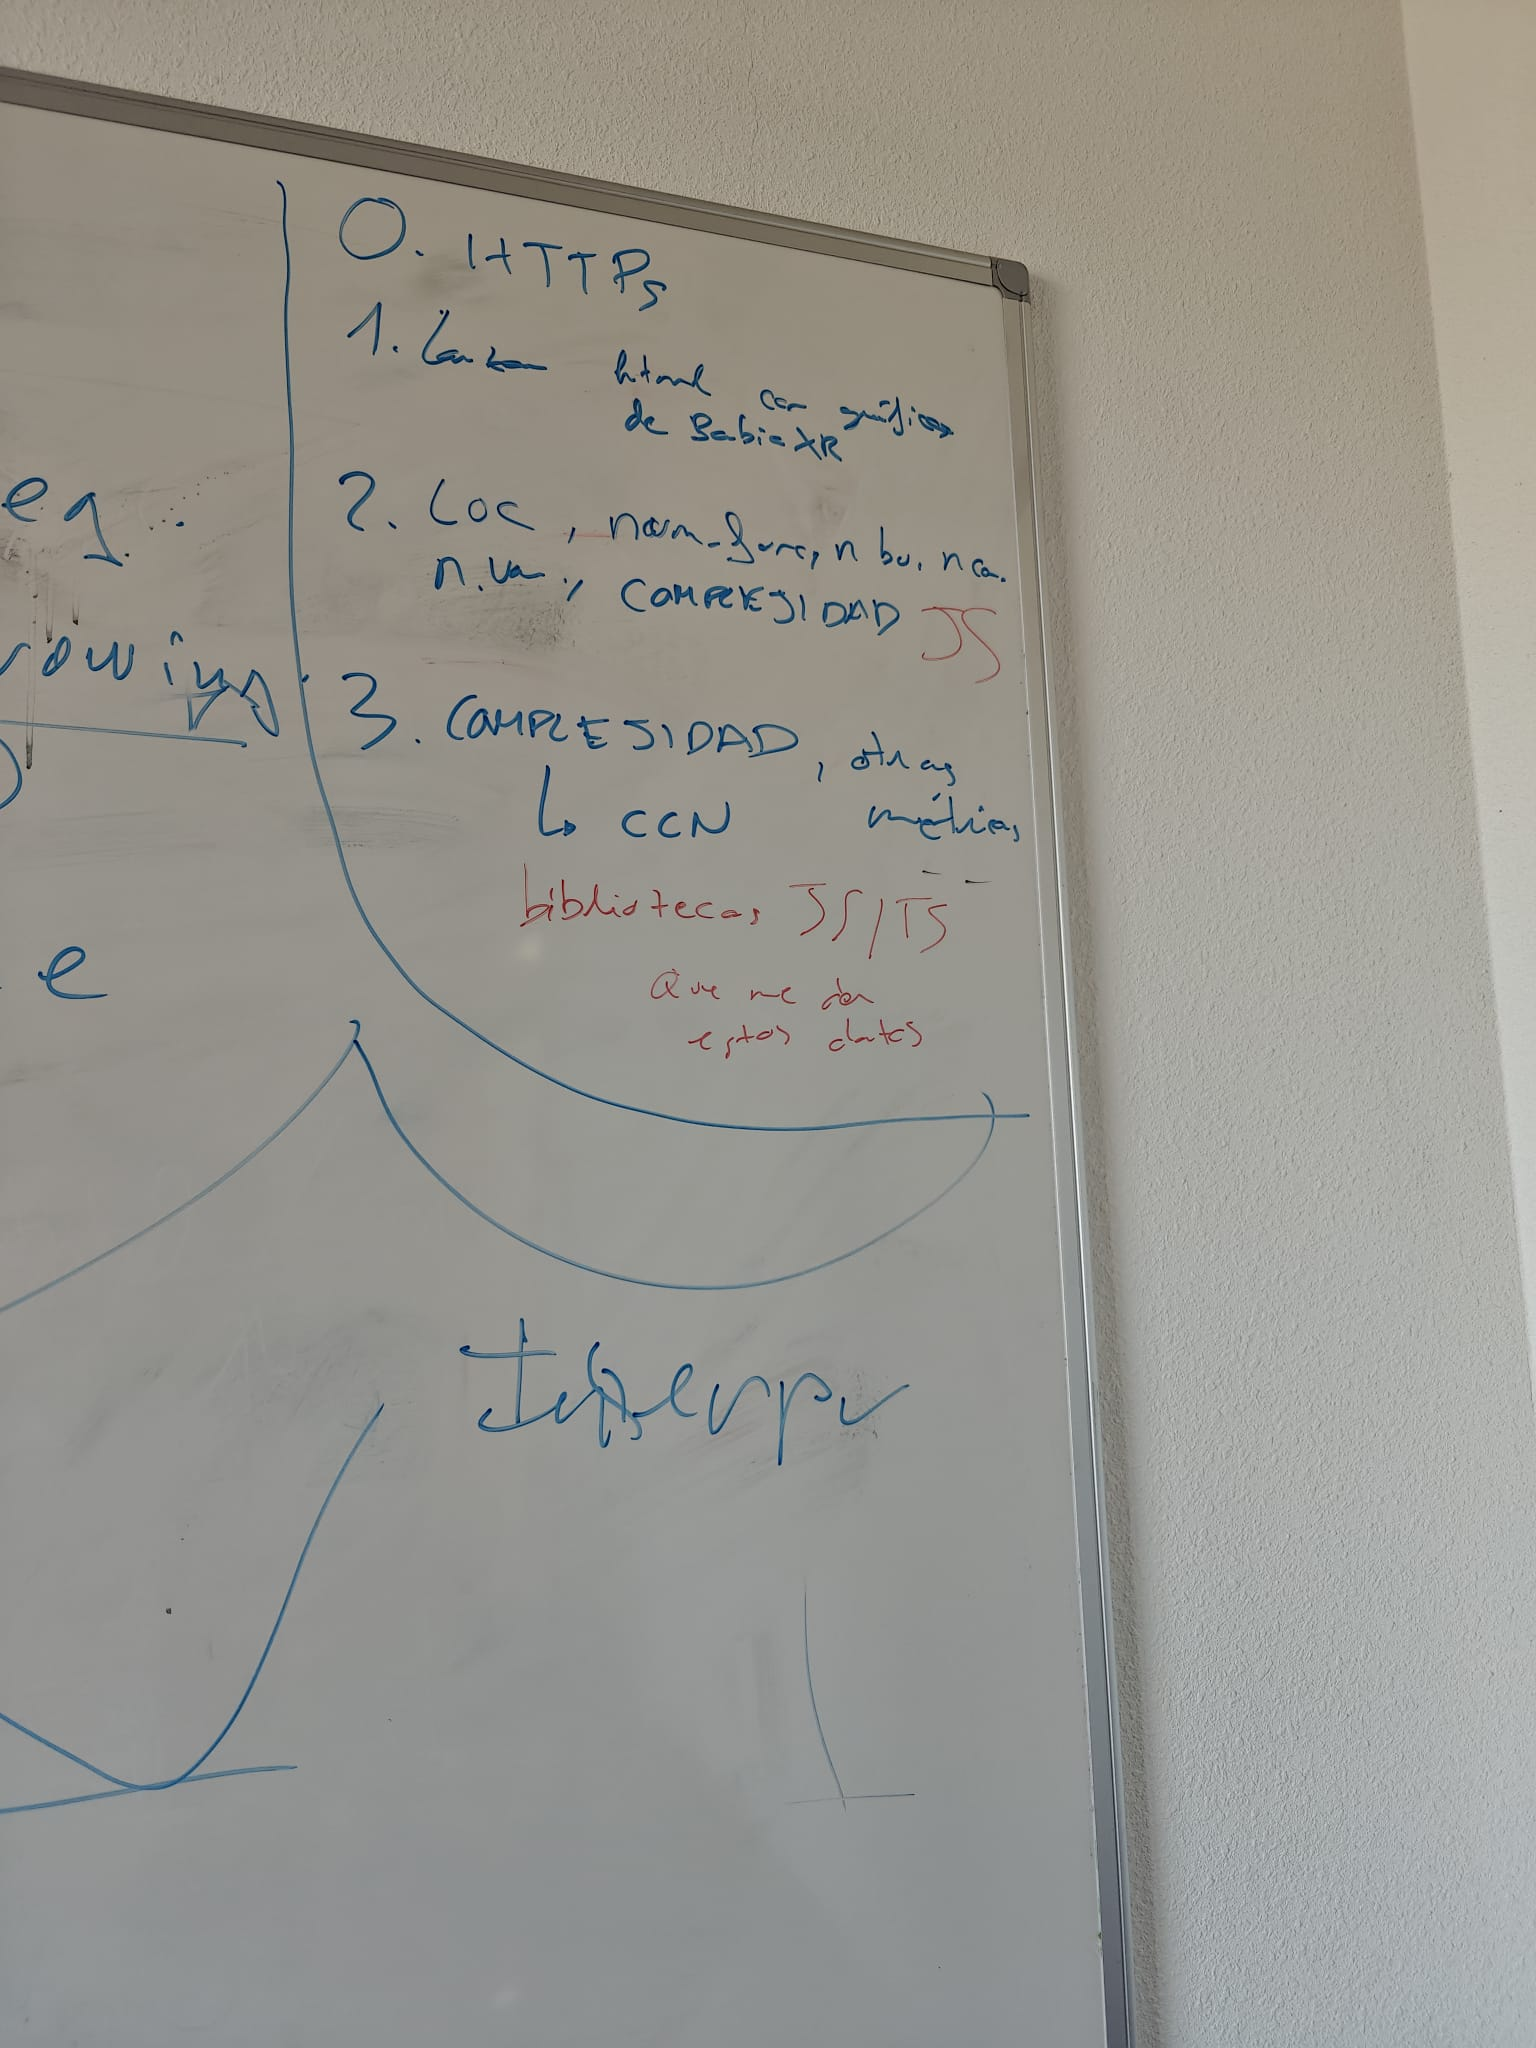
\includegraphics[width=0.8\textwidth]{img/reunion_2025-03-12.png}
    \caption{Imagen de la reunión del 12 de marzo de 2025, donde se definieron los puntos principales del TFG.}
    \label{fig:reunion-marzo}
\end{figure}

%%%%%%%%%%%%%%%%%%%%%%%%%%%%%%%%%%%%%%%%%%%%%%%%%%%%%%%%%%%%%%%%%%%%%%%%%%%%%%%%
%%%%%%%%%%%%%%%%%%%%%%%%%%%%%%%%%%%%%%%%%%%%%%%%%%%%%%%%%%%%%%%%%%%%%%%%%%%%%%%%
% ESTADO DEL ARTE %
%%%%%%%%%%%%%%%%%%%%%%%%%%%%%%%%%%%%%%%%%%%%%%%%%%%%%%%%%%%%%%%%%%%%%%%%%%%%%%%%

\cleardoublepage
\chapter{Estado del arte}
\label{chap:estado}

\section{Visual Studio Code y su sistema de extensiones}
\label{sec:vscode}

Visual Studio Code (VS Code) es un editor de código fuente desarrollado por Microsoft, ampliamente utilizado por la comunidad de desarrolladores debido a su ligereza, extensibilidad y compatibilidad con múltiples lenguajes de programación. Desde su lanzamiento, ha ganado una gran popularidad gracias a características como el autocompletado inteligente, el depurador integrado, la integración con Git y su ecosistema de extensiones.

Una de las características más potentes de VS Code es su sistema de extensiones, que permite ampliar las funcionalidades del editor mediante plugins desarrollados en tecnologías web, principalmente TypeScript, JavaScript, HTML y CSS. Estas extensiones pueden interactuar directamente con el entorno mediante la API oficial de VS Code~\cite{vscode-api}, la cual expone funcionalidades como el acceso al árbol de archivos, la edición del contenido de los documentos, la creación de paneles personalizados, la ejecución de comandos o la escucha de eventos internos del editor.

En el contexto de este Trabajo Fin de Grado, he empleado VS Code no solo como entorno principal de desarrollo, sino también como plataforma de despliegue para la herramienta desarrollada: Code-XR. La elección de esta plataforma ha respondido tanto a motivos técnicos como personales. Por un lado, el ecosistema de extensiones de VS Code permite integrar la visualización de métricas directamente en el entorno de trabajo del programador, lo que evita saltos de contexto y mejora la fluidez del análisis. Por otro lado, se trata del editor que he utilizado a lo largo de toda mi formación universitaria, lo que favorece una mayor familiaridad con su interfaz y flujo de trabajo.

Gracias al uso de la API de extensiones~\cite{vscode-api}, se han podido registrar comandos personalizados, interceptar eventos como la apertura o modificación de archivos y lanzar servidores locales para comunicar el análisis del código con las interfaces XR que forman parte del sistema. El diseño modular de VS Code y su modelo basado en eventos lo convierten en un entorno especialmente adecuado para prototipar herramientas como Code-XR, que requieren integración en tiempo real con el proceso de edición de código.

\section{BabiaXR}
\label{sec:babiaxr}

BabiaXR~\cite{moreno2022babiaxr} es una plataforma de visualización tridimensional e inmersiva desarrollada por investigadores del Grupo de Sistemas y Comunicaciones (GSyC) de la Universidad Rey Juan Carlos (URJC). Está diseñada para facilitar la creación de escenas interactivas en realidad extendida (XR), incluyendo realidad virtual (VR)y aumentada (AR), utilizando tecnologías web abiertas y accesibles como A-Frame, Three.js y WebXR.

El objetivo de BabiaXR es proporcionar un entorno modular y fácilmente integrable que permita a desarrolladores e investigadores visualizar información compleja de forma espacial, sin necesidad de conocimientos avanzados de gráficos 3D. Gracias a su arquitectura basada en componentes personalizables, BabiaXR permite representar datos estructurados como visualizaciones 3D interactivas, directamente desde el navegador y sin necesidad de instalar software adicional. Esto lo convierte en una herramienta especialmente útil en contextos educativos y científicos, donde la simplicidad de despliegue y la portabilidad son factores clave.

En el contexto de este TFG, BabiaXR se ha utilizado como motor base para renderizar las visualizaciones XR de métricas de software generadas por el plugin Code-XR. Concretamente, se han empleado varios de sus componentes gráficos para representar las distintas métricas sobre ficheros o directorios.

\begin{figure}[H]
    \centering
    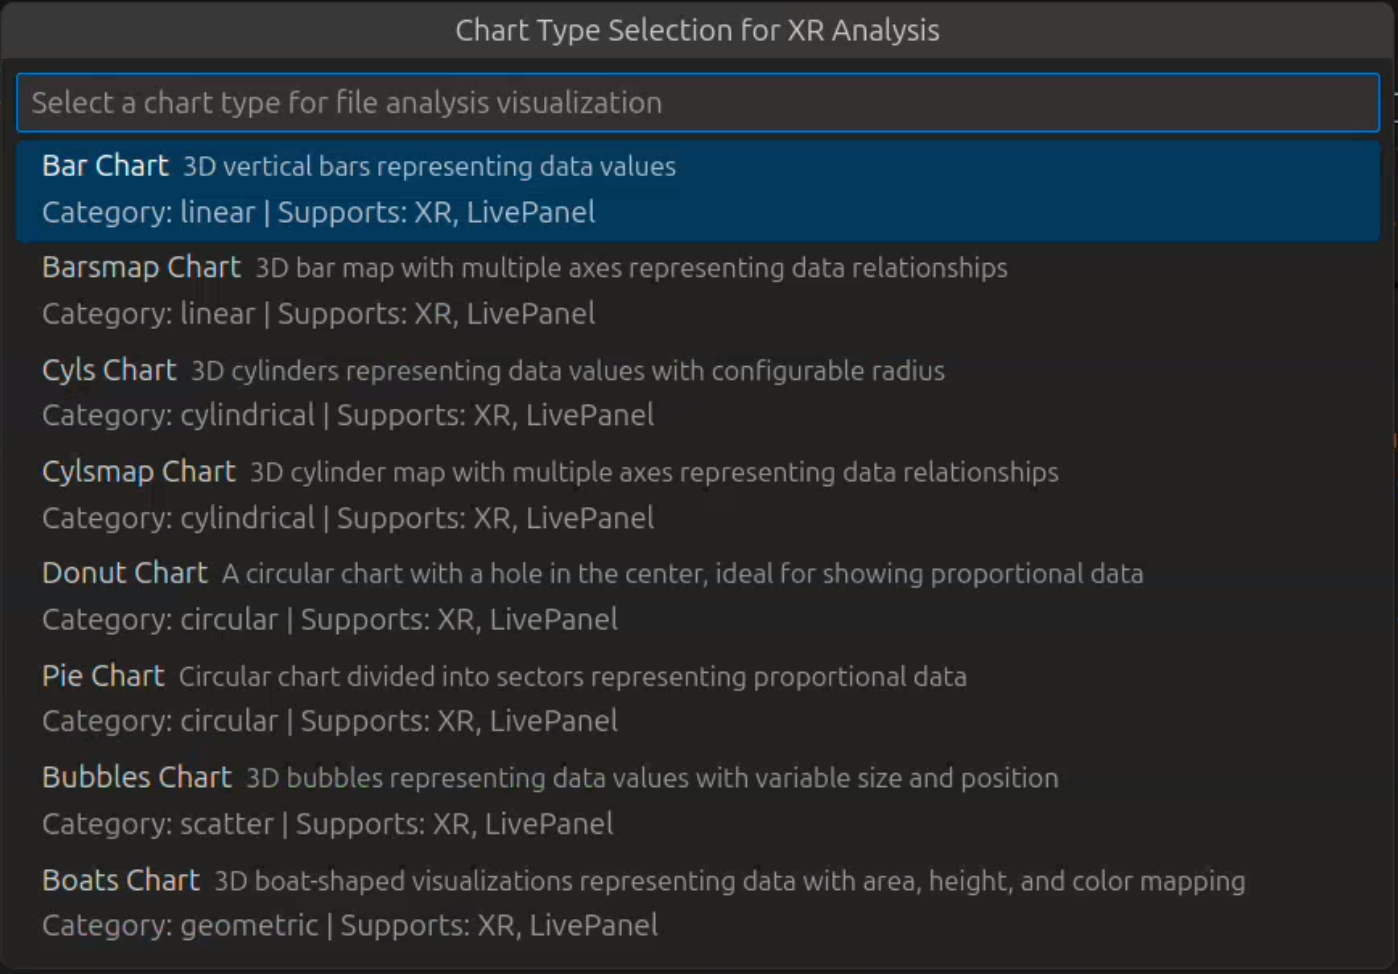
\includegraphics[width=0.85\textwidth]{img/graficos_babiaxr.png}
    \caption{Ejemplo de los diferentes gráficos de BabiaXR utilizados en Code-XR para la visualización de métricas.}
    \label{fig:babiaxr-graficos}
\end{figure}

\section{A-Frame}
\label{sec:aframe}

A-Frame es un framework de código abierto desarrollado inicialmente por Mozilla, orientado a la creación de experiencias inmersivas de realidad virtual y aumentada directamente desde el navegador~\cite{aframe}. Su principal objetivo es reducir la complejidad del desarrollo de escenas 3D, ofreciendo una sintaxis declarativa basada en HTML que permite a los desarrolladores definir entornos tridimensionales mediante etiquetas comprensibles y reutilizables.

Una de las principales ventajas de A-Frame es que se construye sobre Three.js, una biblioteca de bajo nivel para gráficos 3D en WebGL. Gracias a ello, A-Frame ofrece una capa de abstracción que simplifica el uso de luces, cámaras, geometrías y materiales, sin renunciar a la potencia gráfica que subyace bajo el capó. Además, A-Frame está diseñado de forma modular y extensible, lo que permite incorporar componentes personalizados y paquetes externos que enriquecen las capacidades básicas del framework.

En el contexto de este TFG, A-Frame actúa como motor de visualización principal dentro del sistema de representación XR de Code-XR. Toda la escena 3D que se genera al lanzar un análisis con visualización inmersiva —ya sea en modo escritorio o mediante gafas de realidad virtual— está construida como una etiqueta \texttt{<a-scene>} de A-Frame. Dentro de esta escena, se cargan dinámicamente elementos como:

\begin{itemize}
    \item el entorno (\texttt{<a-entity environment=...>}),
    \item los datos obtenidos del análisis (\texttt{<a-entity babia-queryjson=...>}),
    \item los gráficos 3D (como \texttt{<a-entity chart-bar>} o \texttt{<a-entity chart-city>}),
    \item los controladores para interacción con ratón o mandos XR (\texttt{laser-controls}, \texttt{raycaster}, etc.).
\end{itemize}

El sistema también incluye componentes como \texttt{movement-controls}, que permiten al usuario desplazarse libremente por la escena, y \texttt{cursor}, que habilita la interacción mediante puntero en modo escritorio. Esta estructura hace posible una experiencia inmersiva altamente personalizable, donde el usuario puede explorar las métricas del código como si caminara dentro de una ciudad tridimensional interactiva, cambiando parámetros o activando filtros en tiempo real.

Además, se han utilizado extensiones adicionales como:

\begin{itemize}
    \item \textbf{aframe-extras}: para compatibilidad mejorada con mandos y controles de navegación,
    \item \textbf{aframe-environment-component}: para construir entornos virtuales preconfigurados,
    \item \textbf{aframe-geometry-merger-component}: para mejorar el rendimiento gráfico en escenas complejas.
\end{itemize}

Gracias a A-Frame, Code-XR consigue integrar visualización inmersiva XR basada en datos de análisis estático dentro del flujo de trabajo habitual del desarrollador, sin requerir instalaciones externas ni conocimientos especializados de gráficos 3D o motores complejos.


\section{WebXR y Three.js}
\label{sec:webxr-threejs}

WebXR es un estándar impulsado por el World Wide Web Consortium (W3C) que proporciona una interfaz unificada para acceder a dispositivos de realidad virtual (VR) y aumentada (AR) desde navegadores web modernos~\cite{webxr}. Esta API permite detectar dispositivos compatibles —como gafas de realidad virtual, controladores de movimiento o sensores de orientación— y renderizar contenido inmersivo directamente en el navegador, sin necesidad de plugins o instalaciones adicionales.

A diferencia de su predecesor, WebVR, el estándar WebXR está diseñado para cubrir tanto experiencias de realidad virtual como aumentada desde una misma API. Esto facilita el desarrollo de aplicaciones XR multiplataforma que funcionen de manera transparente en dispositivos como las Meta Quest, móviles compatibles con AR o incluso navegadores de escritorio. Gracias a WebXR, los entornos construidos con tecnologías web como A-Frame pueden ejecutarse en modo inmersivo y responder en tiempo real a la posición y orientación del usuario, ofreciendo una experiencia más natural e interactiva.

Aunque WebXR no se ha utilizado de forma directa en el código de Code-XR, sí está presente en la infraestructura base proporcionada por BabiaXR y A-Frame. La capacidad de lanzar visualizaciones XR directamente desde el navegador, y que estas puedan ser exploradas en dispositivos VR, se apoya en el soporte nativo de WebXR ofrecido por las capas subyacentes. Esto permite que el usuario final, sin necesidad de configurar nada adicional, pueda sumergirse en una visualización tridimensional del código simplemente accediendo a una URL generada por el plugin.

Por su parte, Three.js es una biblioteca JavaScript de alto nivel para el renderizado de gráficos 3D en WebGL~\cite{threejs}. Proporciona una interfaz sencilla para trabajar con cámaras, luces, materiales, geometrías y animaciones, y ha sido adoptada como base por muchos frameworks más accesibles como A-Frame. En otras palabras, Three.js actúa como el motor gráfico real que renderiza las escenas construidas en A-Frame, traduciéndolas a instrucciones de bajo nivel ejecutadas en la GPU mediante WebGL.

Aunque en este proyecto tampoco se ha programado directamente sobre la API de Three.js, su papel como capa de renderizado es esencial para que Code-XR pueda mostrar métricas en forma de ciudades tridimensionales, edificios interactivos o jerarquías DOM navegables. Gracias a la madurez y optimización de Three.js, la visualización generada es fluida, compatible con múltiples navegadores y capaz de mantener el rendimiento incluso en escenas complejas con decenas o cientos de elementos renderizados.

En resumen, tanto WebXR como Three.js son tecnologías que, aunque no se han utilizado directamente en el código fuente desarrollado, sustentan gran parte de las capacidades inmersivas y gráficas de Code-XR a través de BabiaXR y A-Frame, y son piezas clave del ecosistema web XR moderno.


\section{HTML}
\label{sec:html}

HTML (HyperText Markup Language) es el lenguaje de marcado fundamental para la estructuración de contenido en la web~\cite{html}. En el contexto de Code-XR, HTML actúa como la base común sobre la que se construyen todas las interfaces visuales de la herramienta, independientemente del modo de análisis utilizado: ya sea LivePanel, XR Mode o VisualizeDOM.

Cada vez que el usuario lanza un análisis, el sistema genera dinámicamente una plantilla HTML que se adapta al modo de visualización elegido. Estas plantillas incluyen la carga de scripts, componentes gráficos, referencias a los datos analizados y configuraciones específicas para el entorno XR o la interfaz 2D. Además, todas estas interfaces se sirven desde un servidor local (localhost), lo que permite que el usuario pueda abrirlas tanto en el navegador como desde un panel dentro del propio Visual Studio Code.

En el caso del modo LivePanel, HTML organiza la presentación de métricas en tablas, tarjetas o paneles interactivos, facilitando una exploración clásica y accesible de la información. Para el modo XR, el documento HTML contiene la escena tridimensional definida mediante A-Frame, donde los elementos \texttt{<a-scene>} y \texttt{<a-entity>} representan funciones o archivos del proyecto como estructuras visuales. En el modo VisualizeDOM, el contenido de un fichero HTML es analizado y su estructura DOM se representa como un árbol navegable en 3D, también dentro de una plantilla HTML generada.

La principal ventaja de utilizar HTML como base es su versatilidad y compatibilidad con el ecosistema web, lo que permite incorporar fácilmente bibliotecas, componentes personalizados y sistemas de interacción. Esta modularidad ha permitido a Code-XR mantener una arquitectura visual consistente, reutilizable y expandible, capaz de adaptarse a distintos modos de visualización sin cambiar la infraestructura técnica subyacente.

\section{TypeScript y JavaScript}
\label{sec:typescript-javascript}

TypeScript es un lenguaje de programación desarrollado por Microsoft que extiende JavaScript con tipado estático opcional y características orientadas a objetos~\cite{typescript}. Se compila a JavaScript y es especialmente útil para desarrollar aplicaciones a gran escala. En el caso de Code-XR, TypeScript actúa como el motor principal del plugin para Visual Studio Code, gestionando tanto la lógica de control como la interacción con la API del editor.

Gracias a su sistema de tipos y su compatibilidad con las definiciones de la API oficial de VS Code, TypeScript permite escribir un código más robusto, mantenible y fácilmente depurable. En este TFG, se ha utilizado para estructurar los comandos del plugin, gestionar los flujos de análisis de ficheros o directorios, lanzar servidores locales, y registrar las distintas vistas disponibles (LivePanel, XR Mode, VisualizeDOM). También se encarga de orquestar cuándo y cómo se genera cada visualización, y de enviar los datos de análisis a las interfaces correspondientes.

Por su parte, JavaScript ha sido el lenguaje utilizado en la parte cliente (frontend) de la herramienta, desempeñando un papel fundamental en la actualización dinámica de las visualizaciones~\cite{javascript}. En particular, es el encargado de implementar el sistema de comunicación en tiempo real mediante Server-Sent Events (SSE). Cada vez que se detecta un cambio en el código fuente, el backend (escrito en TypeScript) actualiza el análisis y envía los datos mediante SSE, que son recibidos en el cliente JavaScript para actualizar la vista correspondiente.

En el caso concreto del modo LivePanel, JavaScript también es responsable de inyectar dinámicamente el contenido HTML que representa las métricas del análisis. Esto incluye la creación y actualización de elementos visuales como tarjetas, tablas o gráficos, en función de los datos recibidos. Gracias a esta lógica dinámica, la vista LivePanel puede reaccionar de forma instantánea a los cambios sin necesidad de recargar la página ni ejecutar ningún código adicional por parte del usuario.

La combinación de TypeScript para el control lógico del plugin y JavaScript para la actualización dinámica del frontend ha permitido construir una herramienta modular, eficiente y altamente interactiva. Ambos lenguajes forman parte del ecosistema web moderno y ofrecen un equilibrio ideal entre rendimiento, facilidad de desarrollo y mantenibilidad del código.

\section{CSS}
\label{sec:css}

CSS (Cascading Style Sheets) es el lenguaje estándar utilizado para definir la presentación visual de documentos HTML~\cite{css}. Permite aplicar estilos a elementos web como colores, fuentes, márgenes, disposición de contenido o animaciones. En el contexto de Code-XR, CSS se utiliza exclusivamente para dar estilo a las interfaces generadas en el modo LivePanel, es decir, en las visualizaciones bidimensionales de métricas de código.

Cuando el usuario selecciona este modo de análisis, el sistema genera dinámicamente una plantilla HTML que contiene las métricas estructurales del código, como líneas de código, complejidad ciclomática o número de parámetros. Es en esa plantilla donde CSS entra en juego para mejorar la presentación de los datos y facilitar su interpretación. Por ejemplo, se utiliza para definir colores distintivos según la complejidad, organizar tarjetas o bloques métricos en una disposición clara, y aplicar estilos adaptativos que permitan visualizar correctamente la información en distintos tamaños de ventana.

Aunque CSS no participa en los modos inmersivos XR ni en la representación tridimensional del DOM, sí cumple un rol importante en la experiencia de usuario cuando se elige una visualización 2D. Gracias a su separación respecto a la lógica de análisis (TypeScript) y de comunicación (JavaScript), el uso de CSS ha permitido mantener una arquitectura limpia y modular, en la que el estilo puede modificarse de forma independiente sin afectar al funcionamiento interno del plugin.

\section{Python y Lizard}
\label{sec:python-lizard}

Python es un lenguaje de programación de alto nivel, ampliamente utilizado en tareas de automatización, análisis de datos y procesamiento de texto~\cite{python}. En el marco de este proyecto, Python ha sido la tecnología seleccionada para realizar el análisis estático del código fuente, es decir, para extraer métricas estructurales que luego son representadas visualmente en los distintos modos de Code-XR.

La elección de Python responde a su sencillez sintáctica, su ecosistema de bibliotecas bien establecido y su capacidad para integrarse fácilmente con otros entornos. En este caso, la ejecución de los scripts de análisis se lanza desde el backend del plugin, escrito en TypeScript, mediante servidores locales. Estos scripts procesan ficheros o directorios del proyecto analizado y generan como salida un fichero JSON con las métricas calculadas.

Para calcular métricas como la complejidad ciclomática (CCN), el número de líneas de código (LOC) o el número de funciones o métodos, se ha utilizado la herramienta Lizard~\cite{lizard}, una biblioteca de análisis estático especializada y compatible con múltiples lenguajes de programación. Lizard permite procesar archivos fuente y devolver una representación estructurada de sus componentes, lo que ha facilitado la integración directa con el sistema de visualización de Code-XR.

Los datos generados por los scripts de Python son consumidos tanto por el modo LivePanel, que los muestra en formato 2D, como por el modo XR, donde se representan como edificios o elementos tridimensionales en una ciudad metafórica. En ambos casos, la estructura JSON permite mapear propiedades del código (como tamaño o complejidad) a atributos visuales como altura, color o volumen.

Además, en el modo VisualizeDOM, Python también cumple una función complementaria: leer el contenido del archivo HTML seleccionado y convertirlo a una cadena de texto. Esta cadena se pasa directamente al componente \texttt{babia-html} de BabiaXR, que se encarga de interpretarla y generar la visualización tridimensional correspondiente.

En conjunto, la combinación de Python y Lizard proporciona una base sólida para la obtención de datos estáticos fiables y bien estructurados, esenciales para alimentar las visualizaciones generadas por Code-XR en todos sus modos de funcionamiento.

\section{Gafas de Realidad Virtual: Meta Quest 3}
\label{sec:meta-quest-3}

Para probar y validar las funcionalidades inmersivas del plugin Code-XR, se han utilizado unas gafas de realidad virtual Meta Quest 3, cedidas temporalmente por la Universidad Rey Juan Carlos. Estos dispositivos permiten ejecutar experiencias de realidad virtual de forma autónoma, gracias a su procesador integrado, sensores de movimiento y capacidad de renderizado gráfico sin necesidad de conexión a un ordenador externo.

Durante el desarrollo, las Meta Quest 3 se han empleado para acceder directamente a las visualizaciones XR generadas por Code-XR, conectándose al servidor local lanzado desde el entorno de desarrollo. Esto ha permitido verificar en entorno real el correcto funcionamiento del modo XR, evaluar la experiencia de usuario y realizar ajustes en la navegación, disposición de los gráficos y rendimiento general de la escena.

El uso de estos dispositivos ha sido clave para validar el comportamiento del sistema en condiciones reales de uso inmersivo, especialmente en lo que respecta a la integración con WebXR y la capacidad de renderizar métricas complejas de código en escenarios tridimensionales navegables.


\section{Apoyo de herramientas de inteligencia artificial}
\label{sec:ia}

Durante el desarrollo del proyecto se ha utilizado el apoyo de herramientas basadas en inteligencia artificial, que han resultado útiles como complemento para resolver dudas técnicas, explorar alternativas de implementación y aprender nuevas tecnologías necesarias para llevar a cabo el trabajo.

En particular, ChatGPT~\cite{chatgpt} ha sido una herramienta de referencia para comprender el funcionamiento de bibliotecas como Lizard (usada para el análisis estático de código) o A-Frame (empleada en la construcción de escenas XR). También ha servido como apoyo a la hora de encontrar enfoques para resolver problemas concretos, mejorar la organización de ciertas secciones del código o redactar documentación técnica con un enfoque más claro y estructurado.

Por otro lado, se ha recurrido a Claude 4~\cite{claude4} para tareas relacionadas con la organización de grandes volúmenes de código. Esto ha sido especialmente útil en este proyecto, cuyo repositorio cuenta con más de 200 ficheros solo en la carpeta \texttt{src/}, sin contar plantillas HTML, archivos CSS o scripts JavaScript asociados.

Estas herramientas no sustituyen el conocimiento técnico ni el razonamiento propio, pero sí han aportado valor como apoyo al desarrollo, ayudando a mejorar la eficiencia y la claridad en distintas partes del proyecto.
% Descripción de las tecnologías que utilizas en tu trabajo. 
% Con dos o tres párrafos por cada tecnología, vale. 
% Se supone que aquí viene todo lo que no has hecho tú.

% Puedes citar libros, como el de Bonabeau et al., sobre procesos estigmérgicos~\cite{bonabeau:_swarm}. 
% Me encantan los procesos estigmérgicos.
% Deberías leer más sobre ellos.
% Pero quizás no ahora, que tenemos que terminar la memoria para sacarnos por fin el título.
% Nota que el \~ \ añade un espacio en blanco, pero no deja que exista un salto de línea. 
% Imprescindible ponerlo para las citas.

% Citar es importantísimo en textos científico-técnicos. 
% Porque no partimos de cero.
% Es más, partir de cero es de tontos; lo suyo es aprovecharse de lo ya existente para construir encima y hacer cosas más sofisticadas.
% ¿Dónde puedo encontrar textos científicos que referenciar?
% Un buen sitio es Google Scholar\footnote{\url{http://scholar.google.com}}.
% Por ejemplo, si buscas por ``stigmergy libre software'' para encontrar trabajo sobre software libre y el concepto de \emph{estigmergia} (¿te he comentado que me gusta el concepto de estigmergia ya?), encontrarás un artículo que escribí hace tiempo cuyo título es ``Self-organized development in libre software: a model based on the stigmergy concept''.
% Si pulsas sobre las comillas dobles (entre la estrella y el ``citado por ...'', justo debajo del extracto del resumen del artículo, te saldrá una ventana emergente con cómo citar.
% Abajo a la derecha, aparece un enlace BibTeX.
% Púlsalo y encontrarás la referencia en formato BibTeX, tal que así:

% {\footnotesize
% \begin{verbatim}
% @inproceedings{robles2005self,
%   title={Self-organized development in libre software:
%          a model based on the stigmergy concept},
%   author={Robles, Gregorio and Merelo, Juan Juli\'an 
%           and Gonz\'alez-Barahona, Jes\'us M.},
%   booktitle={ProSim'05},
%   year={2005}
% }
% \end{verbatim}
% }

% Copia el texto en BibTeX y pégalo en el fichero \texttt{memoria.bib}, que es donde están las referencias bibliográficas.
% Para incluir la referencia en el texto de la memoria, deberás citarlo, como hemos hecho antes con~\cite{bonabeau:_swarm}, lo que pasa es que en vez de el identificador de la cita anterior (bonabeau:\_swarm), tendrás que poner el nuevo (robles2005self).
% Compila el fichero \texttt{memoria.tex} (\texttt{pdflatex memoria.tex}), añade la bibliografía (\texttt{bibtex memoria.aux}) y vuelve a compilar \texttt{memoria.tex} (\texttt{pdflatex memoria.tex})\ldots y \emph{voilà} ¡tenemos una nueva cita~\cite{robles2005self}!

% También existe la posibilidad de poner notas al pie de página, por ejemplo, una para indicarte que visite la página del GSyC\footnote{\url{http://gsyc.es}}.



% \section{Sección 1} 
% \label{sec:seccion1}

% Hemos hablado de cómo incluir figuras.
% Pero no hemos dicho nada de tablas.
% A mí me gustan las tablas.
% Mucho.
% Aquí un ejemplo de tabla, la Tabla~\ref{tab:ejemplo} (siento ser pesado, pero nota cómo he puesto la referencia).

% \begin{table}
%  \begin{center}
%   \begin{tabular}{ | l | c | r |} % tenemos tres colummnas, la primera alineada a la izquierda (l), la segunda al centro (c) y la tercera a la derecha (r). El | indica que entre las columnas habrá una línea separadora.
%     \hline
%     Uno & 2 & 3 \\ \hline % el hline nos da una línea vertical
%     Cuatro & 5 & 6 \\ \hline
%     Siete & 8 & 9 \\
%     \hline
%   \end{tabular}
%   \caption{Ejemplo de tabla. Aquí viene una pequeña descripción (el \emph{caption}, el pie de tabla/figura) del contenido de la tabla. Si la tabla no es autoexplicativa, siempre viene bien aclararla aquí.}
%   \label{tab:ejemplo}
%  \end{center}
% \end{table}

% Hay un sitio en Internet donde puedes diseñar las tablas fácilmente y luego hacer un corta y pega del resultado en tu editor.
% Puedes probarlo en \url{https://www.tablesgenerator.com/}.



%%%%%%%%%%%%%%%%%%%%%%%%%%%%%%%%%%%%%%%%%%%%%%%%%%%%%%%%%%%%%%%%%%%%%%%%%%%%%%%%
%%%%%%%%%%%%%%%%%%%%%%%%%%%%%%%%%%%%%%%%%%%%%%%%%%%%%%%%%%%%%%%%%%%%%%%%%%%%%%%%
% DISEÑO E IMPLEMENTACIÓN %
%%%%%%%%%%%%%%%%%%%%%%%%%%%%%%%%%%%%%%%%%%%%%%%%%%%%%%%%%%%%%%%%%%%%%%%%%%%%%%%%

\cleardoublepage
\chapter{Diseño e implementación}
\label{sec:diseno}

% Aquí viene todo lo que has hecho tú (tecnológicamente). 
% Puedes entrar hasta el detalle. 
% Es la parte más importante de la memoria, porque describe lo que has hecho tú.
% Eso sí, normalmente aconsejo no poner código, sino diagramas.



% \section{Arquitectura general} 
% \label{sec:arquitectura}

% Si tu proyecto es un software, siempre es bueno poner la arquitectura (que es cómo se estructura tu programa a ``vista de pájaro'').

% \begin{figure}
%   \centering
%   \includegraphics[width=9cm, keepaspectratio]{img/arquitectura.png}
%   \caption{Estructura del parser básico}
%   \label{fig:arquitectura}
% \end{figure}


% Por ejemplo, puedes verlo en la figura~\ref{fig:arquitectura}.
% \LaTeX \ pone las figuras donde mejor cuadran. 
% Y eso quiere decir que quizás no lo haga donde lo hemos puesto\ldots 
% Eso no es malo.
% A veces queda un poco raro, pero es la filosofía de \LaTeX: tú al contenido, que yo me encargo de la maquetación.


 
% Recuerda que toda figura que añadas a tu memoria debe ser explicada.
% Sí, aunque te parezca evidente lo que se ve en la figura~\ref{fig:arquitectura}, la figura en sí solamente es un apoyo a tu texto.
% Así que explica lo que se ve en la figura, haciendo referencia a la misma tal y como ves aquí.
% Por ejemplo: En la figura~\ref{fig:arquitectura} se puede ver que la estructura del \emph{parser} básico, que consta de seis componentes diferentes: los datos se obtienen de la red, y según el tipo de dato, se pasará a un \emph{parser} específico y bla, bla, bla\ldots

% Si utilizas una base de datos, no te olvides de incluir también un diagrama de entidad-relación.


\section{Arquitectura general} 
\label{sec:arquitectura}

En esta sección se presenta la arquitectura general de Code‑XR, explicando sus componentes principales, los canales de comunicación entre ellos y las decisiones tecnológicas que sustentan su diseño. El objetivo es ofrecer una visión global suficiente para entender cómo fluye la información desde el código fuente hasta las visualizaciones en 2D (LivePanel) y XR.

En los siguientes apartados de este capítulo se explicará cómo se desarrollaron las distintas partes del plugin, los pasos o sprints seguidos durante el desarrollo y cómo se estableció la comunicación entre los componentes, incluyendo detalles sobre protocolos, formatos de intercambio y la orquestación entre TypeScript, Python y las vistas cliente.


\subsection{Componentes y responsabilidades}
\begin{itemize}
  \item \textbf{VS Code Extension (TypeScript):} registro de comandos, UI en el editor, gestión de procesos (lanzamiento de servidores HTTP/HTTPS, análisis con Python mediante entorno virtual, etc...), y almacenamiento de configuraciones. En conclusión, TypeScript es el lenguaje que maneja toda la lógica del plugin a través de la API oficial de Visual Studio Code~\cite{vscode-api}.
  \item \textbf{Python metrics engine:} ejecución de scripts en Python para el análisis estático de ficheros y directorios. La mayor parte de las métricas se extraen usando la librería Lizard~\cite{lizard}, mientras que algunas métricas complementarias se calculan mediante código Python propio. El resultado se normaliza y se exporta en formato JSON para ser entendido por los componentes de BabiaXR~\cite{moreno2022babiaxr}.
  \item \textbf{JSON Storage / Manager:} formato intermedio y almacenamiento temporal de resultados (ficheros .json o memoria). Este formato se utiliza tanto para las configuraciones del plugin —por ejemplo, parámetros a representar y el tipo de gráfico seleccionado— como para la salida de los análisis ejecutados por Python (las métricas se exportan en JSON). Las configuraciones persistentes del plugin se guardan usando la API de VS Code en globalState (ExtensionContext.globalState), de modo que se mantienen entre sesiones del editor; por su parte, los resultados de análisis y datos asociados al proyecto se almacenan en workspaceState (ExtensionContext.workspaceState), que queda ligado al workspace abierto y no se comparte entre workspaces. Para más detalles sobre ambos mecanismos de almacenamiento véase la documentación oficial de VS Code~\cite{vscode-storage}.
  \item \textbf{Realtime API (SSE):} canal unidireccional basado en Server‑Sent Events (SSE) para enviar actualizaciones incrementales de métricas a los clientes (LivePanel, XR). En el cliente se implementa mediante la API nativa `EventSource` de JavaScript, y en el servidor mediante respuestas HTTP con content‑type \texttt{text/event-stream}~\cite{mdn-sse}. 

  Aunque existen librerías como express-sse~\cite{express-sse} que facilitan la implementación de SSE en aplicaciones Node.js, se optó por una implementación nativa para mantener un control granular sobre los eventos enviados y reducir las dependencias externas del plugin. El sistema funciona de la siguiente manera: cuando un fichero observado cambia, la extensión detecta la modificación, lanza un re‑análisis (entorno virtual de Python), normaliza y actualiza el JSON correspondiente en workspaceState, y emite eventos SSE específicos como \texttt{analysis-updated} o \texttt{dataRefresh}. Los clientes suscritos (LivePanel, páginas XR) escuchan estos eventos mediante \texttt{EventSource('/events')}, reciben las notificaciones y actualizan automáticamente las visualizaciones sin recargar la página.
  \item \textbf{Servidores de visualización (HTML/CSS/JS):} conjunto de plantillas web servidas por servidores locales HTTP/HTTPS para la visualización de métricas. Incluye dos modos principales:
  \begin{itemize}
    \item \textbf{LivePanel}: webview embebida en VS Code para visualización 2D con tablas, gráficos y métricas detalladas.
    \item \textbf{XR Pages}: escenas 3D basadas en A-Frame y BabiaXR para visualización inmersiva en navegador o dispositivos VR.
  \end{itemize}
  Ambos modos comparten la misma infraestructura de servidor y comunicación SSE. Para el acceso desde dispositivos XR (como Meta Quest 3), el servidor debe configurarse en modo HTTPS con certificados autofirmados generados mediante OpenSSL~\cite{openssl}, ya que los navegadores en dispositivos VR requieren conexiones seguras para acceder a las APIs de WebXR.
  \item \textbf{Sistema de plantillas dinámicas:} generador automático de plantillas HTML específicas para cada tipo de análisis y visualización. Incluye procesamiento de placeholders, validación de dimensiones de datos, y adaptadores para diferentes gráficos BabiaXR según el tipo de métricas extraídas.
  \item \textbf{File watcher y detección de cambios:} monitorización automática de archivos para re-análisis en tiempo real. Utiliza la API de VS Code para detectar modificaciones en los ficheros bajo análisis y triggear actualizaciones automáticas del JSON y las vistas asociadas.
  \item \textbf{Registry de servidores activos:} sistema de registro y gestión del ciclo de vida de servidores HTTP/HTTPS lanzados por el plugin. Permite controlar múltiples instancias simultáneas, gestionar puertos dinámicos y evitar conflictos entre diferentes análisis en ejecución.
\end{itemize}


% ...existing code...
\subsection{Tipos de análisis}
\label{sec:tipos-analisis}

A continuación se presenta una tabla simplificada con los tipos fundamentales de análisis soportados por Code‑XR, su alcance y si admiten la opción \emph{deep} (recursión por subdirectorios) o la posibilidad de aplicarse al workspace completo (análisis de proyecto).

\begin{figure}[H]
\centering\small
\begin{tabular}{p{5.0cm} p{7.5cm} p{2.5cm}}
\hline
\textbf{Tipo de análisis} & \textbf{Alcance} & \textbf{Deep? / Proyecto?} \\
\hline
Fichero — LivePanel & Análisis puntual de un único fichero; visualización 2D en el panel integrado. & No / No \\
Fichero — XR & Análisis puntual de un único fichero; representación inmersiva en A‑Frame/BabiaXR. & No / No \\
Directorio — LivePanel & Análisis de un directorio; resumen por archivo y agregados por carpeta. & Sí / Sí \\
Directorio — XR & Representación 3D del contenido de un directorio (escena A‑Frame/BabiaXR). & Sí / Sí \\
DOM Mode (especial) & Análisis de la estructura DOM de un fichero HTML; visualización 3D específica del DOM. & No / No \\
\hline
\end{tabular}
\caption{Tipos fundamentales de análisis, alcance y soporte de \emph{deep}/\emph{proyecto}.}
\label{tab:tipos-analisis}
\end{figure}

\bigskip

\noindent Para mayor claridad, a continuación se muestra la relación entre los comandos expuestos en la interfaz (menú contextual / editor) y el tipo de análisis que lanzan.


\begin{figure}[H]
\centering\small
\begin{tabular}{p{9.0cm} p{6.0cm}}
\hline
\textbf{Comando (UI)} & \textbf{Identificador interno / Tipo} \\
\hline
CodeXR: Analyze File (LivePanel) & \texttt{newCodeAnalysis.analyzeFile} — Fichero / LivePanel \\
CodeXR: Analyze File (XR) & \texttt{newCodeAnalysis.analyzeFileXR} — Fichero / XR \\
CodeXR: Analyze Directory (LivePanel) & \texttt{newCodeAnalysis.analyzeDirectory} — Directorio / LivePanel (No deep) \\
CodeXR: Analyze Directory (LivePanel Deep) & \texttt{newCodeAnalysis.analyzeDirectoryDeep} — Directorio / LivePanel (Deep) \\
CodeXR: Analyze Directory (XR) & \texttt{newCodeAnalysis.analyzeDirectoryXR} — Directorio / XR (No deep) \\
CodeXR: Analyze Directory (XR Deep) & \texttt{newCodeAnalysis.analyzeDirectoryXRDeep} — Directorio / XR (Deep) \\
CodeXR: Analyze Project (LivePanel) & \texttt{newCodeAnalysis.analyzeProject} — Proyecto / LivePanel (raíz del workspace) \\
CodeXR: Analyze Project (LivePanel Deep) & \texttt{newCodeAnalysis.analyzeProjectDeep} — Proyecto / LivePanel (Deep, raíz del workspace) \\
CodeXR: Analyze Project (XR) & \texttt{newCodeAnalysis.analyzeProjectXR} — Proyecto / XR (raíz del workspace) \\
CodeXR: Analyze Project (XR Deep) & \texttt{newCodeAnalysis.analyzeProjectXRDeep} — Proyecto / XR (Deep, raíz del workspace) \\
CodeXR: Visualize DOM & \texttt{newCodeAnalysis.visualizeDOM} — DOM Mode \\
\hline
\end{tabular}
\caption{Mapeo entre comandos de la UI y tipos de análisis (incluye variantes de proyecto).}
\label{tab:comandos-analisis}
\end{figure}

\bigskip


Notas:
\begin{itemize}
  \item Los comandos de ``Proyecto'' operan reutilizando la misma lógica interna que los comandos de ``Directorio''; la única diferencia es que, al invocarse, toman la raíz del workspace como directorio a analizar.
  \item La forma de invocar estos comandos desde la interfaz es mediante el menú contextual (click derecho) en el explorador de archivos o en el editor. La asignación de entradas de menú, reglas de visibilidad y los identificadores de comando están declarados en el fichero \texttt{package.json} del plugin; en un apartado posterior se detalla la estructura y funcionamiento de \texttt{package.json} en extensiones de VS Code. Otra forma también de invocarlos es a través de un acceso rápido integrado en la interfaz del plugin, que permite seleccionar ficheros y directorios mediante las vistas ``Files by Language'' y ``Project Structure''. Esto se explicará con más detalle en la sección dedicada a la interfaz del plugin.
  \item ``Deep'' indica análisis recursivo sobre subdirectorios; su uso incrementa la cantidad de datos y las entidades en la escena XR, por lo que puede requerir optimizaciones de rendimiento (batching, análisis incremental, reducción de nivel de detalle).
\end{itemize}


\section{Flujo de datos / Secuencia de ejecución}
\label{sec:flujo-ejecucion}


A continuación se explica, de forma general y sin referencias a rutas concretas, la secuencia básica que sigue un análisis en Code‑XR desde la petición del usuario hasta la actualización de la visualización. Esta descripción está pensada para ofrecer una visión global del flujo de trabajo.

\begin{enumerate}
  \item \textbf{Petición del análisis.} El usuario solicita un análisis mediante la interfaz gráfica (clic derecho), a través del menú rápido del plugin (\emph{Files by Language} o \emph{Project Structure}) o ejecutando el comando desde la paleta de comandos (F1). La petición especifica el tipo de análisis deseado y el objetivo (ruta al fichero o al directorio a analizar).
  \item \textbf{Registro de la sesión de análisis.} Se crea una sesión de análisis con un identificador único (nonce) y se registran los datos necesarios para ejecutar y rastrear el análisis: la ruta de almacenamiento en el directorio \texttt{workspaceStorage} (ver \cite{vscode-storage}), la lista de ficheros involucrados, el tipo de análisis, el estado actual de la sesión y los parámetros de configuración. Tras crear la sesión, el flujo continúa con la obtención de los ficheros necesarios para el análisis.
  \item \textbf{Obtención de los ficheros necesarios.} Según el tipo de análisis, el motor determina los ficheros y parámetros necesarios para ejecutar y presentar el resultado: las plantillas HTML/CSS/JS que se usarán en la vista, y los argumentos con los que ejecutar el script principal \texttt{main.py} que realizará el análisis para generar el fichero \texttt{data.json} con las métricas. En la práctica se prepara un paquete compuesto por la plantilla HTML, los recursos CSS/JS y el fichero de datos; adicionalmente se copia un \texttt{favicon.ico} para la interfaz (no relevante para la lógica del análisis). Todos estos ficheros se guardan en la ruta de almacenamiento creada para la sesión dentro del directorio \texttt{workspaceStorage}. El parseado de la plantilla HTML cambia según el tipo de análisis solicitado (p. ej. LivePanel vs XR); el detalle del parseado se describe en la sección dedicada a explicar cómo funciona el análisis de Code‑XR.
  \item \textbf{Persistencia temporal de la sesión.} Una vez generado el paquete con todos los datos necesarios, éstos se guardan en la ruta indicada para la sesión. Esta persistencia facilita el re\-análisis y el arranque del servidor de visualización. Los ficheros resultantes de los análisis realizados durante la sesión se eliminan de \texttt{workspaceStorage} al cerrar VS Code, evitando así dejar \emph{analysis zombies} que ocupen espacio innecesario.
  \item \textbf{Activación de watchers con debounce.} Se registran observadores (watchers) sobre los ficheros implicados para detectar cambios. Los watchers aplican un \emph{debounce time}: un intervalo configurable que sirve para agrupar eventos de cambio que ocurren en rápida sucesión (por ejemplo, mientras un desarrollador escribe). En ausencia de debounce, cada modificación podría disparar un nuevo análisis y generar sobrecarga; con debounce, el sistema espera hasta que no se producen más cambios durante el intervalo configurado y entonces ejecuta el análisis, evitando re\-análisis innecesarios. Si el usuario cambia dinámicamente el valor del \emph{debounce time} durante una sesión, los watchers se reconfiguran para emplear el nuevo intervalo inmediatamente, afectando a las detecciones posteriores.
  \item \textbf{Lanzamiento del servidor de visualización y canal SSE.} Se inicia un servidor local que sirve los ficheros HTML/CSS/JS preparados para la sesión como `localhost` (o `https://localhost` si el usuario tiene configurado HTTPS). La forma concreta de arrancar el servidor (puerto, HTTP/HTTPS, certificados, etc...) depende de la configuración del usuario; en cualquier caso el servidor expone además un canal de eventos en tiempo real mediante Server‑Sent Events (SSE) que se utiliza para notificar a las vistas cuando hay resultados nuevos tras un re‑análisis.
  \item \textbf{Detección de cambios y re‑análisis incremental.} Cuando un watcher detecta un cambio en un fichero, se siguen estos pasos:
    \begin{enumerate}[label=\alph*), nosep, topsep=0pt, partopsep=0pt, parsep=0pt, itemsep=0.5ex, leftmargin=2em]
      \item Identificar la sesión de análisis asociada al fichero modificado.
      \item Re‑analizar únicamente los ficheros afectados (análisis incremental) y actualizar el JSON/metadata de la sesión.
      \item Persistir los resultados en la ruta de la sesión para que el servidor los sirva inmediatamente.
      \item Emitir un evento por el canal SSE (\texttt{analysis-updated}); las vistas suscritas reciben la notificación y actualizan la visualización en tiempo real.
    \end{enumerate}
\end{enumerate}

% Diagrama vertical en TikZ
\begin{figure}[H]
\centering
\begin{tikzpicture}[
  node distance=8mm,
  procstep/.style={rectangle, draw=black, rounded corners, fill=gray!10, text width=10.5cm, align=center, minimum height=10mm},
  arr/.style={-{Stealth}, thick}
]
\node[procstep] (p1) {1. Petición del análisis};
\node[procstep, below=of p1] (p2) {2. Registro de la sesión};
\node[procstep, below=of p2] (p3) {3. Obtención de ficheros};
\node[procstep, below=of p3] (p4) {4. Persistencia temporal};
\node[procstep, below=of p4] (p5) {5. Watchers (debounce)};
\node[procstep, below=of p5] (p6) {6. Servidor + SSE};
\node[procstep, below=of p6] (p7) {7. Detección y re‑análisis};
\draw[arr] (p1) -- (p2);
\draw[arr] (p2) -- (p3);
\draw[arr] (p3) -- (p4);
\draw[arr] (p4) -- (p5);
\draw[arr] (p5) -- (p6);
\draw[arr] (p6) -- (p7);
\end{tikzpicture}
\caption{Secuencia vertical simplificada del flujo de un análisis.}
\label{fig:flujo-vertical}
\end{figure}

\noindent En el siguiente diagrama se ofrece una visión abstracta y lineal del proceso. En la práctica, varias sesiones pueden coexistir, teniendo para un fichero mas de un watcher activo (p. ej. un análisis de directorio y otro de proyecto que incluyan el mismo fichero). El sistema gestiona estas situaciones mediante el registro de sesiones y watchers, asegurando que cada cambio se propaga correctamente a todas las vistas afectadas.

% Explicacion de la evolucion del proyecto
% ...existing code...
\section{Resumen cronológico de versiones}
\label{sec:resumen-versiones}
A continuación se presenta un resumen cronológico compacto de las versiones principales del plugin (desde la 0.0.1 hasta la 1.0.0). La tabla está ordenada empezando por la versión inicial (0.0.1) y finalizando en la versión estable (1.0.0). En la subsección siguiente se describirán con más detalle los sprints/hitos relacionados con estas versiones.

\begin{table}[H]
\centering\small
\begin{tabular}{p{2.2cm} p{2.8cm} p{9.0cm}}
\hline
\textbf{Versión} & \textbf{Fecha (aprox.)} & \textbf{Resumen / hito principal} \\
\hline
0.0.1 & 2025-03-11 & Primer prototipo: servidor HTTP que servía un HTML A‑Frame predefinido (prueba de concepto XR) y comandos básicos para lanzar la visualización. \\
0.0.2 & 2025-03-20 & Primer análisis básico en modo LivePanel para ficheros JavaScript/TypeScript; ya se comenzó a controlar la infraestructura XR (selección del HTML a servir y primeras comprobaciones de HTTPS), pero las visualizaciones principales seguían siendo 2D (LivePanel). \\
0.0.3 & 2025-04-11 & Introducción de auto‑reanalysis, selección inteligente de ejes, integración SSE, watchers por fichero y primer soporte de análisis estático (LOC, CCN, funciones). \\
0.0.4 & 2025-04-27 & Soporte multi‑lenguaje ampliado y sistema configurable de debounce para auto‑análisis; mejoras en XR y análisis múltiple simultáneo. \\
0.0.5 & 2025-04-29 & Nuevas visualizaciones (babia‑boats), mapeo de parámetros a dimensiones visuales y mejoras en plantillas y resolución de rutas. \\
0.0.6 & 2025-04-29 & Publicación inicial en marketplace: estabilización de servidores, UX y preparación para distribución pública. \\
0.0.7 & 2025-06-01 & Mejora del live reload y experiencia XR: SSE robusto, controles VR/AR mejorados y configuración avanzada de entornos. \\
0.0.8 & 2025-07-03 & Revisión mayor del motor de análisis: soporte Lizard ampliado, Visualize DOM, nuevas visualizaciones (bubble chart) y optimizaciones de watcher/caché. \\
0.0.9 & 2025-07-27 & Re‑arquitecturación del motor de análisis: análisis de directorios completos, soporte deep y mejoras de rendimiento/fiabilidad. \\
1.0.0 & 2025-07-28 & Versión estable: sistema de auto-análisis configurable, gestión avanzada de sesiones con prevención de duplicados, filtrado inteligente de ficheros HTML, optimización de configuración y watchers, y publicación de la web oficial de documentación (https://amontesl.github.io/code-xr-docs/). \\
\hline
\end{tabular}
\caption{Resumen cronológico de versiones — hitos principales (orden: 0.0.1 → 1.0.0).}
\label{tab:changelog}
\end{table}


\noindent Nota: los detalles en esta tabla se han extraído y condensado desde el fichero \texttt{CHANGELOG.md}. Hay registros públicos en \texttt{CHANGELOG.md} a partir de la versión 0.0.3; el plugin estuvo publicado en el marketplace desde la versión 0.0.6. Las fechas aproximadas indican momentos representativos del desarrollo y se usan para situar cronológicamente los hitos.


% Diagrama temporal simplificado de la evolución de versiones
\begin{figure}[H]
  \centering
  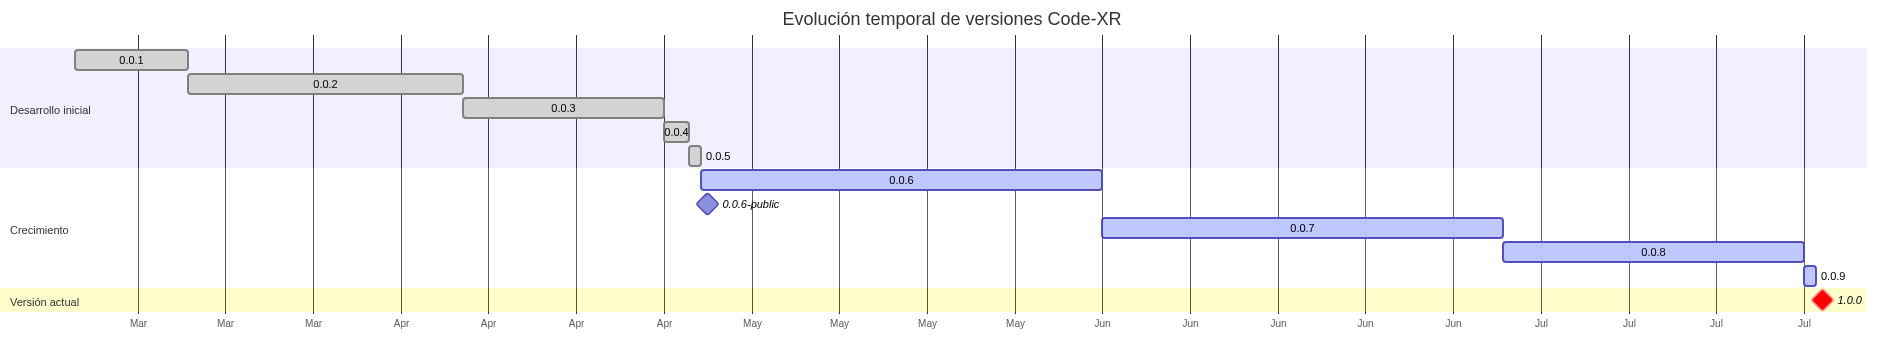
\includegraphics[width=\textwidth]{img/versions_gantt.png}
  \caption{Evolución temporal resumida de las versiones principales del proyecto.}
  \label{fig:timeline-versions}
\end{figure}
% ...existing


\noindent En los siguientes subapartados se describirán los sprints/hitos que explican cómo se pasó de la idea inicial a la versión 1.0.0, detallando para cada sprint el objetivo, las tareas realizadas y los artefactos resultantes.



\section{Primeros pasos}
\label{sec:primeros-pasos}

Esta sección recoge los conceptos básicos y decisiones iniciales adquiridos durante la creación de la extensión para VS Code. El propio editor ofrece un tutorial introductorio para desarrollar una primera extensión\cite{tutorialVSCode}, el cual se siguió en paralelo con recursos en vídeo, como el tutorial oficial de VS Code en YouTube\cite{vscode-youtube}. A partir de estos materiales, y utilizando el generador oficial de extensiones (``Yo Code'')\cite{yo-code}, se establecieron las bases del proyecto y se tomaron las primeras decisiones técnicas que marcaron su desarrollo inicial.

\subsection{Generador \emph{Yo Code}}
El generador oficial de extensiones para VS Code, denominado ``Yo Code'', guía al desarrollador mediante una serie de preguntas que definen la plantilla inicial del plugin: identificador y nombre de la extensión, descripción, publicador, lenguaje de desarrollo (TypeScript o JavaScript), inicialización opcional de un repositorio Git, gestor de paquetes y el tipo de empaquetado (opciones típicas: \emph{unbundled}, Webpack, Esbuild). Estas decisiones iniciales configuran la estructura base del proyecto y los scripts para compilar, empaquetar y desplegar la extensión.

\subsection{Elección de lenguaje}
Se optó por \textbf{TypeScript}, dado que ofrece tipado estático que reduce errores, integración directa con las definiciones de la API de VS Code y mayor mantenibilidad en proyectos de mediana y gran escala\cite{typescript}. Este lenguaje permitió a Code-XR evolucionar de forma segura al crecer en número de ficheros y complejidad.

\subsection{Bundlers}
El proceso de empaquetado de una extensión de VS Code puede realizarse de distintas formas, dependiendo del flujo de desarrollo y de los requisitos de distribución. La documentación oficial recomienda evaluar diferentes bundlers según las necesidades del proyecto\cite{vscode-bundling}.  
Entre las opciones más habituales se incluyen:
\begin{itemize}
  \item \textbf{Unbundled}: sin bundler, útil para prototipado rápido pero obliga a distribuir dependencias manualmente.
  \item \textbf{Webpack}: bundler clásico y ampliamente usado; genera un único paquete y minimiza dependencias externas\cite{webpack}.
  \item \textbf{Esbuild}: bundler moderno, extremadamente rápido y con tiempos de compilación reducidos\cite{esbuild}.
\end{itemize}

En Code-XR se comenzó con la plantilla \emph{unbundled} para acelerar el prototipado y validar la integración con A-Frame y BabiaXR. Posteriormente se migró a un flujo con \textbf{Webpack}, que sigue siendo el bundler activo en la actualidad. El cambio no solo aportó mayor fiabilidad en la distribución, sino que también resolvió limitaciones prácticas: en versiones recientes, el empaquetado a formato \texttt{.vsix} generaba advertencias de \texttt{npm} por tamaño excesivo. Con Webpack, dichas advertencias desaparecieron y los tiempos de compilación se redujeron de forma notable.

\subsection{Archivo \texttt{package.json} (manifiesto de la extensión)}
El fichero \texttt{package.json} es el manifiesto central de toda extensión de VS Code. Contiene los metadatos que identifican la extensión en el Marketplace (nombre, versión, publicador, categorías, icono y repositorio), además de la compatibilidad con el motor de VS Code y la lista de ficheros incluidos en la distribución.  

También controla el proceso de compilación y empaquetado mediante la sección \texttt{scripts}, que en Code-XR se apoya en Webpack para generar un bundle reproducible siguiendo las recomendaciones oficiales\cite{vscode-bundling}.  

Otra sección clave es \texttt{contributes}, donde se definen los elementos que la extensión añade a la interfaz: más de 40 comandos, la vista lateral \texttt{codexrTree}, y menús contextuales en el explorador, el editor y las vistas de elementos. Esta configuración conecta la extensión con el usuario final y organiza la navegación.  

En cuanto a \texttt{activationEvents}, Code-XR declara una lista vacía, lo que implica activación ansiosa al abrir VS Code. Aunque lo recomendable es activar bajo demanda (\texttt{onCommand}, \texttt{onView}, \texttt{onLanguage}), esta decisión garantizó que todos los menús y vistas estuviesen disponibles desde el inicio.  

Finalmente, la \textbf{iconografía} de la extensión se construyó principalmente con \emph{Codicons}, la librería oficial de VS Code\cite{codicons}. Se emplearon iconos de \emph{Devicon}\cite{devicon} para representar ficheros en vistas como \emph{Files per Language} y \emph{Project Structure}, mientras que el logotipo de Code-XR se generó de manera personalizada mediante técnicas de inteligencia artificial.

\subsection{Archivo \texttt{extension.ts}}
El archivo \texttt{extension.ts} implementa la lógica declarada en el manifiesto. Es el punto de entrada de la extensión y define dos funciones fundamentales:  
\begin{itemize}
  \item \texttt{activate}: se ejecuta al activar la extensión y orquesta la inicialización de servicios (gestión de servidores, restauración de configuraciones, limpieza automática de análisis obsoletos), el registro de la vista modular (\texttt{codexrTree}), la asociación de comandos y la sincronización del estado de visualización de datos.  
  \item \texttt{deactivate}: se invoca al desactivar la extensión y garantiza la liberación ordenada de recursos, como servidores activos, gestores SSE, mapeos de ficheros y vistas modulares.  
\end{itemize}

En Code-XR, este fichero asegura que la extensión arranque en un estado limpio y predecible, y que al cerrarse no queden procesos en segundo plano ni recursos bloqueados.

\subsection{Registro de comandos e interfaz de usuario}
El registro de comandos es el mecanismo que conecta las acciones del usuario con la lógica implementada en la extensión. Cada comando se declara en \texttt{package.json} y se enlaza en \texttt{extension.ts} mediante su \emph{handler}. En Code-XR, los comandos abarcan desde el análisis de ficheros y directorios hasta la gestión de servidores y ejemplos de BabiaXR.  

La interfaz de usuario se apoya en primitivas de la API de VS Code como:
\begin{itemize}
  \item \textbf{TreeView / TreeDataProvider}: para organizar servidores, ejemplos y análisis activos en la vista lateral.
  \item \textbf{WebviewPanel} y \textbf{WebviewView}: para mostrar visualizaciones interactivas en 2D (LivePanel) o XR.
  \item \textbf{StatusBarItem} y elementos contextuales: para notificaciones rápidas y accesos directos.
\end{itemize}

Estas primitivas permitieron a Code-XR ofrecer una experiencia integrada en el flujo habitual del editor, combinando menús, paneles y vistas enriquecidas en una misma extensión.

\begin{figure}[H]
\centering
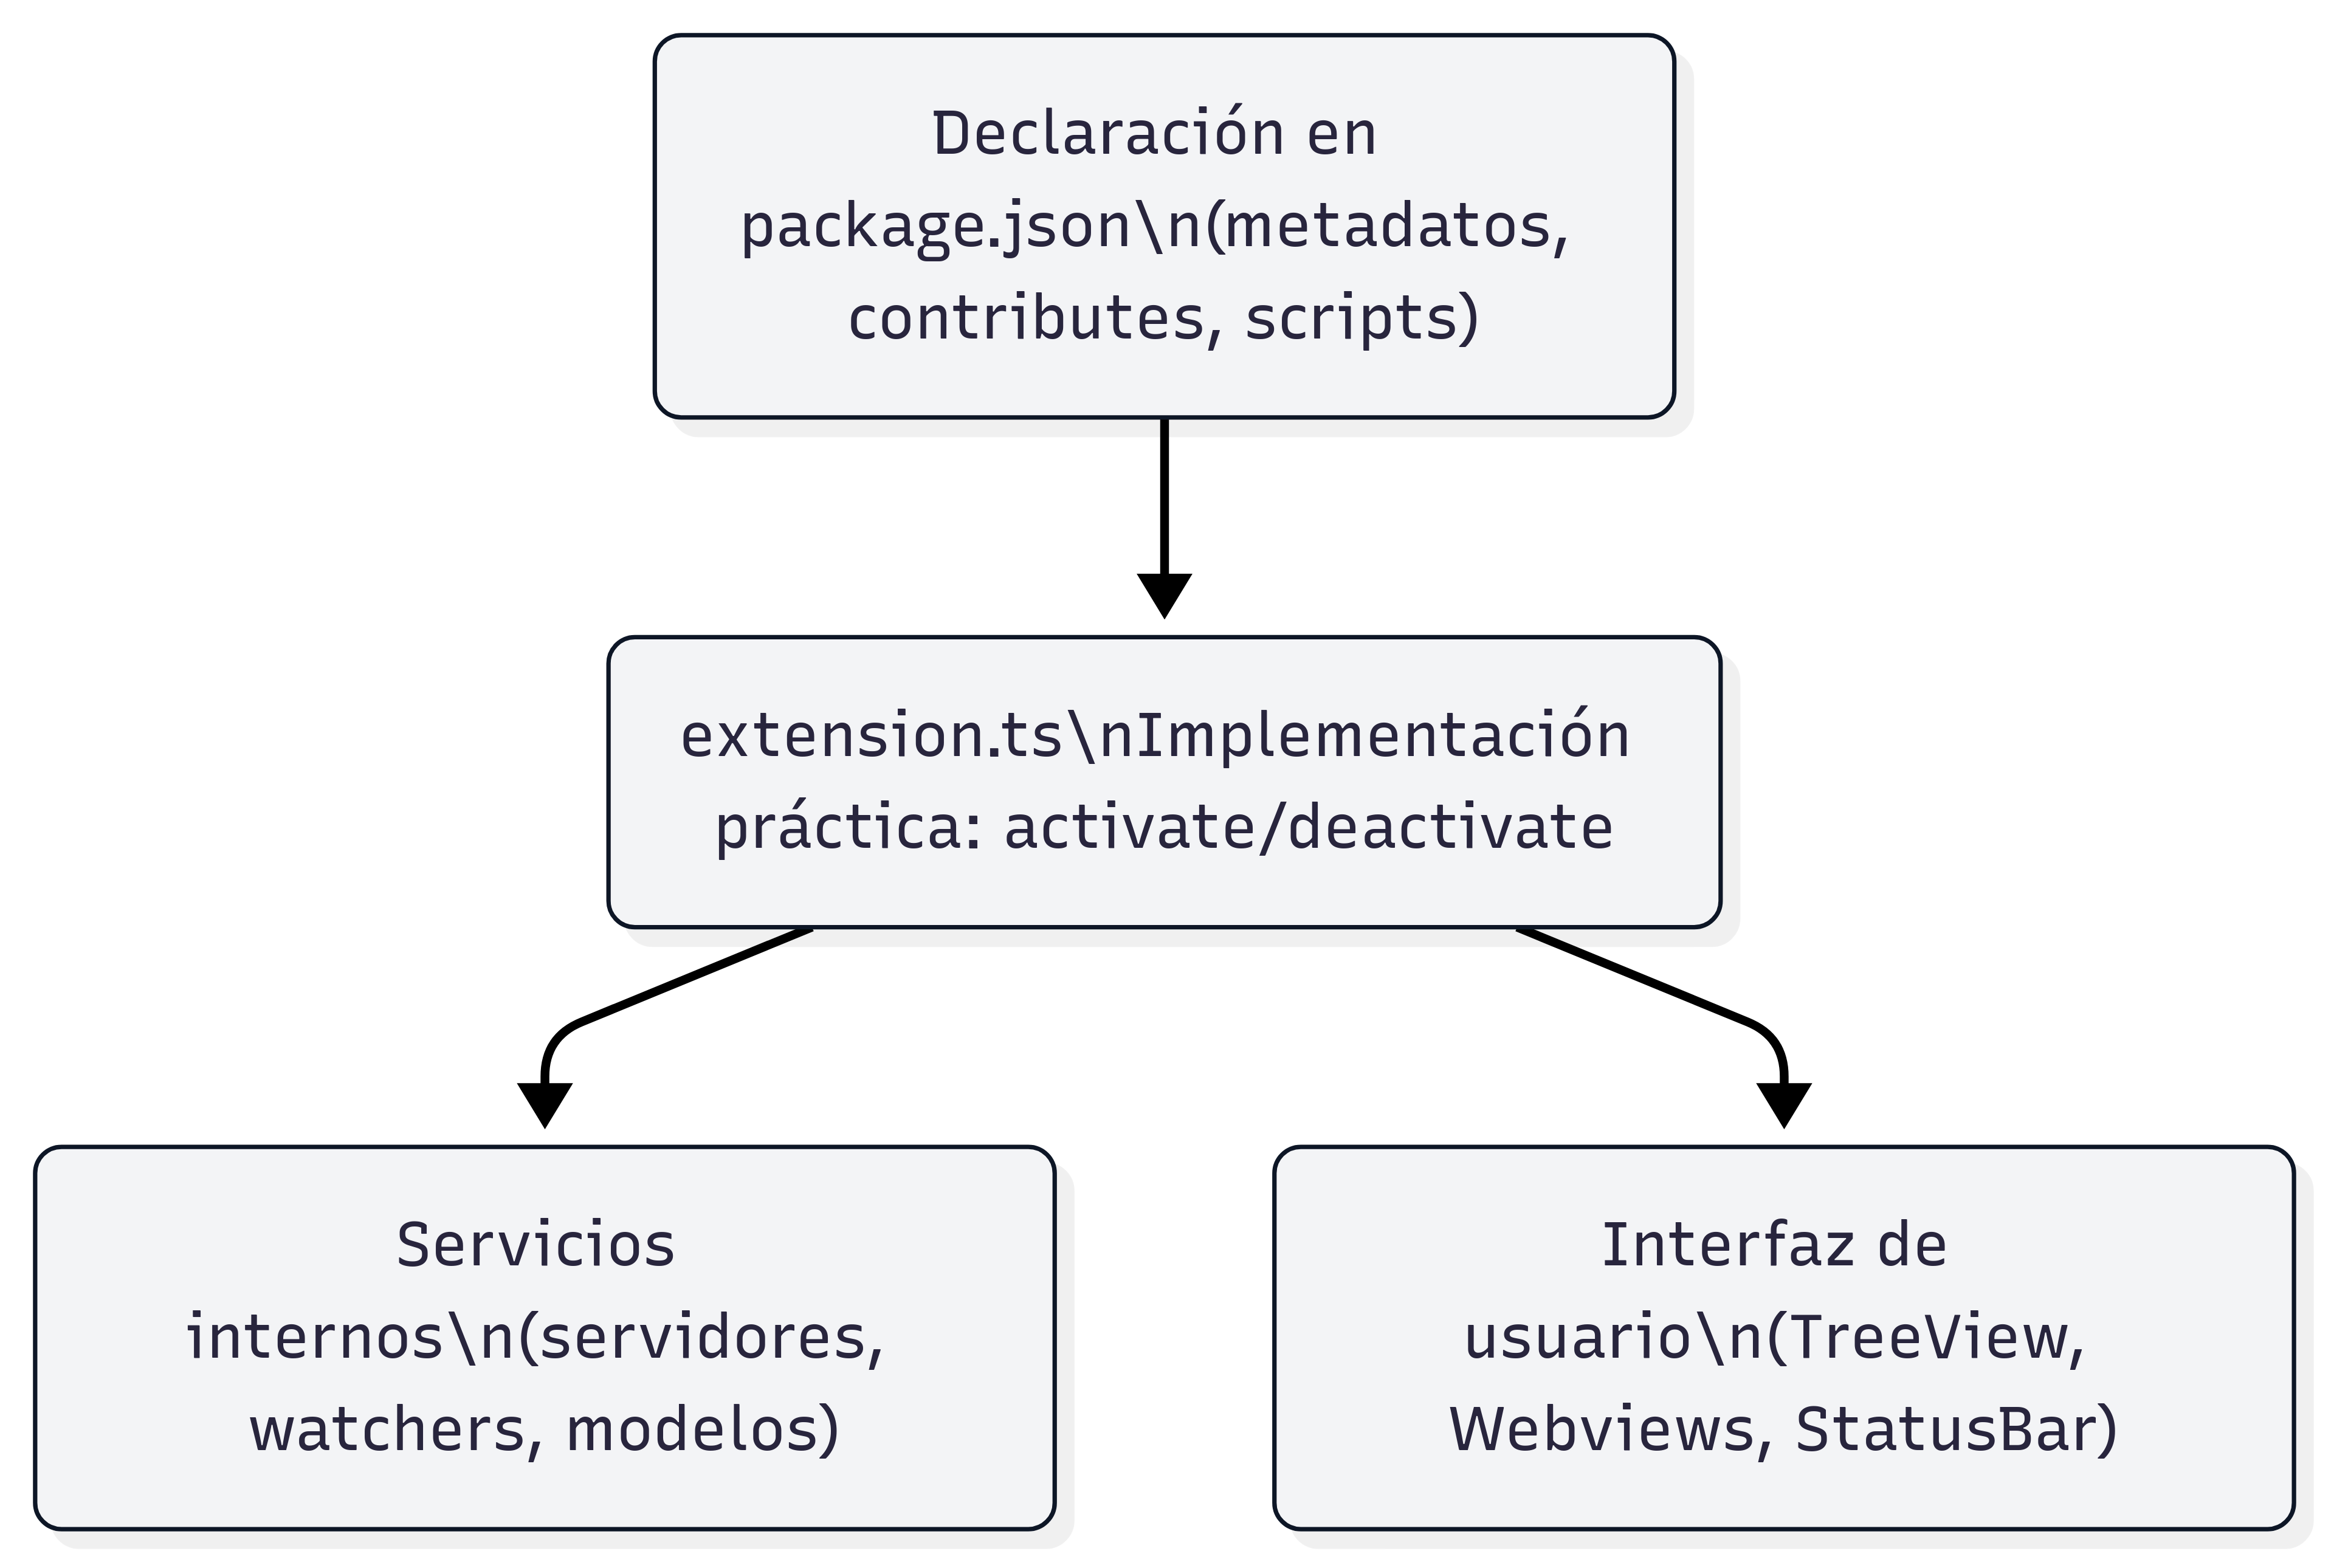
\includegraphics[width=0.8\linewidth]{img/fig-extension-structure.png}
\caption{Relación entre los componentes clave de una extensión VS Code en Code-XR.}
\label{fig:extension-structure}
\end{figure}

% SECCION DE SPRINTS

\section{Sprint 1 — Lanzamiento de servidores locales}
\label{sec:sprint-servers}

Introducción. Este fue el primer objetivo planteado para poner en marcha Code-XR: dotar a la extensión de la capacidad de lanzar servidores locales en \emph{localhost}, permitiendo que los recursos de la extensión pudieran servirse de manera accesible desde un navegador o desde la propia interfaz del editor. La idea se inspiraba en el funcionamiento de otras extensiones consolidadas como \emph{Live Server}\cite{liveserver}, que facilitan un flujo de trabajo más ágil al eliminar la necesidad de configurar manualmente un servidor externo.  

\subsection{Primeras versiones — lanzamiento de servidores}
En las primeras versiones el servidor era mínimamente funcional: servía un HTML fijo con una escena A‑Frame de ejemplo (prueba de concepto) y ofrecía comandos básicos para arrancar y parar la visualización desde la paleta de comandos. Posteriormente se fueron incorporando capacidades incrementales:

\begin{itemize}
  \item selección del fichero HTML a servir en lugar de usar una plantilla fija;
  \item Control de múltiples servidores y gestión automática de puertos: la extensión incorporó la librería \texttt{get-port}\cite{get-port}, que permite detectar de forma dinámica puertos disponibles en el sistema. De este modo se evitaba la colisión con puertos ya ocupados y se garantizaba que cada servidor local pudiera lanzarse sin interferencias. Además, este mecanismo facilitó la reutilización de puertos en sesiones posteriores cuando resultaba apropiado, proporcionando una experiencia más fluida y predecible para el usuario.
  \item Soporte HTTPS: se añadió la posibilidad de lanzar los servidores en modo seguro utilizando certificados por defecto incluidos en la extensión el par \texttt{cert}/\texttt{key} ubicado en la carpeta interna \texttt{certs} preparados con \texttt{OpenSSL}\cite{openssl}. Como alternativa, el usuario puede seleccionar sus propios certificados autofirmados mediante el explorador de ficheros, indicando las rutas de \texttt{cert} y \texttt{key}. Esta doble modalidad (certificados internos frente a certificados personalizados) aporta flexibilidad y facilita la adopción de HTTPS en distintos entornos sin complicar el flujo de lanzamiento.
\end{itemize}

Llegados a este punto de mínima funcionalidad, con la capacidad de servir los servidores en modo HTTPS, se pudo dar por concluido el primer hito y avanzar hacia las siguientes etapas del desarrollo. No obstante, antes de continuar, en la próxima subsección se detalla el estado actual del sistema de lanzamiento de servidores, tanto en lo referente a la interfaz de usuario como a su funcionamiento interno dentro del plugin.

\subsection{Versión actual — lanzamiento y gestión de servidores}
\label{sec:sprint-servers-current}

En la versión actual de Code-XR, el subsistema de servidores proporciona un entorno robusto para servir visualizaciones con \textbf{arquitectura modular}, \textbf{persistencia de preferencias}, \textbf{multi-servidor concurrente}, \textbf{resolución automática de puertos}, \textbf{soporte HTTPS completo} y \textbf{gestión centralizada de estado}. El diseño sigue patrones de desarrollo escalables con separación clara de responsabilidades y gestión de ciclo de vida automatizada, a continuación se detallan los componentes clave, para detalles mas específicos ver el código fuente en el repositorio\cite{code-xr}.

\paragraph{Arquitectura modular del subsistema}
El código se estructura en capas especializadas bajo \texttt{src/servers/} y \texttt{src/active\_servers/}, implementando una arquitectura de responsabilidades distribuidas:

\begin{itemize}
  \item \textbf{runtime}: Núcleo de ejecución con \texttt{httpServer.ts}, \texttt{httpsDefaultServer.ts}, \texttt{httpsCustomServer.ts}, \texttt{multiServerLauncher.ts}, \texttt{portManager.ts} y subsistema \texttt{sse/} para comunicación bidireccional.
  \item \textbf{storage}: \texttt{serverSettingsManager.ts} implementa persistencia con \emph{deep merge}, validación atómica y migraciones de esquema.
  \item \textbf{registry}: \texttt{activeServerRegistry.ts} (singleton) gestiona el estado centralizado con eventos síncronos para UI.
  \item \textbf{services}: \texttt{serverRegistrar.ts} valida registros, \texttt{panelManager.ts} controla WebviewPanels del editor.
  \item \textbf{views}: Integración con TreeView gracias a \texttt{ActiveServersSectionProvider.ts}.
\end{itemize}



\paragraph{Configuración y persistencia (globalStorage)}
El \texttt{ServerSettingsManager} (patrón singleton) gestiona preferencias mediante archivo JSON \texttt{server-settings.json} guardado en \texttt{globalStorage} usando \texttt{context.globalStorageUri}, garantizando \textbf{persistencia cross-workspace}. Cuando el usuario cambia la configuracion ya sea usando la interfaz del UI o a través de comandos el fichero se actualiza automáticamente. La estructura de configuración consta con los siguientes campos:

\begin{figure}[H]
\centering
\begin{minipage}{0.9\linewidth}
\begin{lstlisting}[language=json,
caption={Ejemplo del archivo \texttt{server-settings.json} que persiste la configuración de servidores en Code-XR.},
label={fig:server-settings-json}]
{
  "mode": "HTTPS",
  "https": { "certSource": "default",
             "certPath": "certs/babia_cert.pem",
             "keyPath":  "certs/babia_key.pem" },
  "defaultPort": 3000,
  "launch": { "autoOpen": true, "openMode": "browser" },
  "configNonce": "37a3047821ba23de99348bcba2d155c3",
  "version": "1.0.0"
}
\end{lstlisting}
\end{minipage}
\end{figure}


El \texttt{configNonce} (SHA-256) previene corrupción en actualizaciones concurrentes, mientras que \texttt{version} permitiría hacer migraciones si el esquema cambia en futuras versiones.

\paragraph{UI de configuración avanzada}
El panel de configuración (Figura~\ref{fig:ui-server-config}) expone controles granulares: selección \textbf{HTTP/HTTPS} con validación de certificados, configuración de \textbf{puerto por defecto} con verificación de disponibilidad, es decir, se buscara un puerto libre desde el selecionado por defecto, \textbf{apertura automática} configurable, \textbf{modo de lanzamiento} (panel VS Code vs navegador), funciones de \textbf{reset/restore} y lanzamiento directo con la configuración activa.

\begin{figure}[H]
\centering
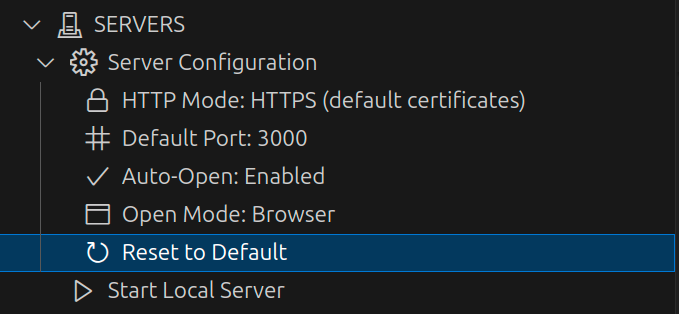
\includegraphics[width=0.55\linewidth]{img/ui-server-config.png}
\caption{Panel de configuración avanzada de servidores en Code-XR con validación en tiempo real.}
\label{fig:ui-server-config}
\end{figure}

\paragraph{Multi-servidor concurrente y gestión inteligente de puertos}
El \texttt{MultiServerLauncher} orquesta \textbf{instancias concurrentes} con identificadores únicos (\texttt{server-\{port\}-\{timestamp\}}), tipado fuerte (\texttt{http | https-default | https-custom}) y metadatos completos (puerto, archivo servido, registro activo). El \texttt{PortManager} implementa descubrimiento automático de puertos mediante:

\begin{enumerate}
  \item Verificación de disponibilidad en puerto preferido usando bind a \texttt{0.0.0.0}
\item Resolución automática de colisiones mediante la librería \texttt{get-port}\cite{get-port}, que realiza una búsqueda secuencial desde el puerto por defecto configurado hasta el rango superior (8080), seleccionando el primer puerto disponible.
  \item Fallback manual con límites configurables y notificación al usuario
  \item Soporte multi-puerto para servicios paralelos
\end{enumerate}

Ante colisiones, el sistema notifica transparentemente la reasignación: \emph{``Puerto 3000 ocupado, servidor lanzado en puerto 3001''}.

\paragraph{HTTPS y gestión de certificados}
El soporte HTTPS implementa dos modalidades con validación previa:

\begin{itemize}
  \item \textbf{Certificados por defecto}: Par \texttt{cert/key} incluido en \texttt{certs/} (generados con \texttt{OpenSSL}\cite{openssl}), permitiendo HTTPS inmediato sin configuración.
  \item \textbf{Certificados personalizados}: Selector de archivos con validación de compatibilidad OpenSSL, rutas absolutas y verificación de integridad antes del lanzamiento.
\end{itemize}

El sistema detecta automáticamente conflictos \textbf{HTTPS + panel lateral} (incompatibilidad de seguridad VS Code) y sugiere apertura del servidor en navegador web con un mensaje contextual.

\paragraph{Active Servers: registro centralizado y observabilidad}
La vista \emph{Active Servers} expone un \textbf{registro centralizado} (\texttt{ActiveServerRegistry}, singleton con patrón Observer) que rastrea instancias activas con:

\begin{itemize}
  \item \textbf{Estado completo}: ID único, puerto, URL, modo de lanzamiento, certificados, timestamp, estado (\texttt{running|stopped|error}).
  \item \textbf{Metadatos contextuales}: Archivo servido, nombre personalizado, sesión de análisis asociada, configuración de red.
  \item \textbf{Etiquetado inteligente}: Prioridad \texttt{customName} $\rightarrow$ \texttt{localhost:port}, descripción con \texttt{launchMode} y indicadores de estado.
  \item \textbf{Acciones contextuales}: \emph{Open in Browser}, \emph{Open in Panel} (solo HTTP), \emph{Copy URL} (local/red), \emph{Stop}, \emph{Server Details} y \emph{Stop All} (disponible con 2+ servidores).
  \item \textbf{Iconografía diferenciada}: Globe (HTTP), Shield (HTTPS-default), Shield-check (HTTPS-custom) con colorimetría por estado (verde/gris/rojo).
\end{itemize}

El registro es \textbf{efímero} (no persiste entre sesiones) para prevenir servidores zombie y garantizar coherencia de entorno (puertos disponibles, interfaces de red, certificados válidos).

\begin{figure}[H]
\centering
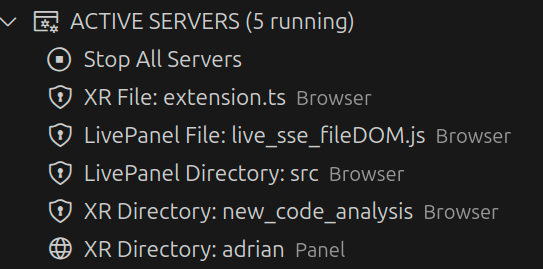
\includegraphics[width=0.62\linewidth]{img/ui-active-servers.png}
\caption{Vista \emph{Active Servers}: registro centralizado con acciones contextuales y estado en tiempo real.}
\label{fig:ui-active-servers}
\end{figure}

\paragraph{Comunicación en tiempo real (SSE) y sincronización}
Los servidores exponen endpoints \texttt{/events} con \emph{Server-Sent Events} (SSE) que implementan:

\begin{itemize}
  \item \textbf{Propagación automática}: Cambios de análisis, actualizaciones de datos y eventos de sistema sin polling.
  \item \textbf{Gestión de clientes}: Registro/limpieza automática de conexiones SSE por archivo analizado.
  \item \textbf{Mapeo archivo-servidor}: Asociación directa entre sesiones de análisis y servidores activos para updates dirigidos.
  \item \textbf{Bus de comunicación}: El servidor actúa como intermediario entre extensión y visualizaciones web.
\end{itemize}

\paragraph{Integración con análisis y limpieza automática}
El sistema implementa \textbf{limpieza coordinada} entre componentes:

\begin{enumerate}
  \item \textbf{Parada de servidor}: Cierra paneles laterales, limpia clientes SSE, elimina mapeos archivo-servidor, cierra sesiones de análisis asociadas.
  \item \textbf{Gestión de ciclo de vida}: Validación periódica de estado, detección de servidores zombie, recovery automático de errores.
  \item \textbf{Sincronización UI}: Eventos del registro activo actualizan TreeView en tiempo real, comandos VS Code integrados.
  \item \textbf{Cleanup de extensión}: Liberación ordenada de todos los recursos al desactivar Code-XR.
\end{enumerate}

\paragraph{Acceso de red y compatibilidad VR/móvil}
El \texttt{NetworkUtils} detecta automáticamente la IP local y genera URLs de acceso externo, facilitando el uso desde dispositivos VR o móviles en la misma red. Los servidores se configuran con bind a \texttt{0.0.0.0} (todas las interfaces) y proporcionan diagnósticos de red para troubleshooting.

\paragraph{Síntesis técnica}
El subsistema combina \textbf{arquitectura modular escalable}, \textbf{configuración persistente con validación}, \textbf{multi-servidor concurrente robusto}, \textbf{gestión inteligente de puertos}, \textbf{HTTPS} y \textbf{registro centralizado con observabilidad}. La integración completa con VS Code (TreeView, comandos, paneles) y el canal SSE bidireccional posicionan este módulo como la columna vertebral técnica de Code-XR, proporcionando una base sólida para el ecosistema de visualización XR.

%----------------------------------------------------------------
% Sprint 2 - BabiaXR
%----------------------------------------------------------------

\section{Sprint 2 — Integración con BabiaXR y ejemplos de visualización}
\label{sec:sprint-babiaxr}

El segundo sprint marcó la transición de Code-XR desde un sistema capaz de lanzar servidores locales hacia una extensión con funcionalidades de visualización XR completas y operativas. Para alcanzar el objetivo principal del plugin mostrar análisis de ficheros y directorios en formato XR inmersivo era fundamental primero comprender y dominar la librería \textbf{BabiaXR}, que constituye el motor de visualización 3D sobre el que se construyen todas las representaciones WebXR/AR/VR de Code-XR.

El desarrollo siguió una progresión lógica y pedagógica dividida en tres fases consecutivas, cada una construyendo sobre los conocimientos y capacidades establecidas en la anterior:

\paragraph{Fase 1: Comprensión de BabiaXR mediante ejemplos}
La primera aproximación consistió en crear una galería de ejemplos predefinidos que permitiera explorar y entender las capacidades fundamentales de BabiaXR. Este enfoque facilitó la familiarización con los diferentes tipos de gráficos disponibles (barras, sectores, burbujas, cilindros, etc.), sus parámetros de configuración, las estructuras de datos requeridas y las mejores prácticas para integrar A-Frame con componentes BabiaXR en el contexto de una extensión VS Code.

\paragraph{Fase 2: Conexión de datos JSON con visualizaciones}
Una vez establecida una base sólida de comprensión sobre BabiaXR, el siguiente paso natural fue desarrollar la capacidad de transformar datos arbitrarios en formato JSON en visualizaciones interactivas. Esta fase requirió diseñar e implementar un pipeline completo de procesamiento que abarcara desde el análisis automático de estructuras de datos hasta la generación dinámica de plantillas HTML/A-Frame, pasando por el mapeo inteligente de campos de datos a dimensiones visuales específicas de cada tipo de gráfico.

\paragraph{Fase 3: Personalización y control visual}
La fase final se centró en proporcionar al usuario control granular sobre los aspectos estéticos y ambientales de las visualizaciones generadas. Esto incluyó la implementación de un sistema de configuración que permitiera seleccionar ambientes 3D (bosques, paisajes futuristas, entornos abstractos), personalizar colores de fondo y suelo, y elegir paletas cromáticas optimizadas para diferentes tipos de datos y contextos de visualización.

Esta aproximación incremental no solo facilitó el desarrollo técnico, sino que también estableció una base arquitectónica sólida y extensible para futuras mejoras del sistema de visualización XR.

\paragraph{Módulos resultantes}
El sprint produjo tres subsistemas especializados e interconectados:
\begin{enumerate}
  \item \textbf{Babia Examples}: galería interactiva de ejemplos predefinidos BabiaXR que sirve como plataforma de aprendizaje y punto de partida para nuevas visualizaciones.
  \item \textbf{Visualize Data}: pipeline sofisticado de transformación que convierte datos JSON arbitrarios en visualizaciones XR mediante flujo guiado, análisis automático de campos y mapeo inteligente de dimensiones.
  \item \textbf{Visualization Settings}: sistema de configuración visual que permite personalizar ambientes 3D, esquemas de color, paletas de gráficos y otros parámetros estéticos aplicados globalmente a todas las visualizaciones.
\end{enumerate}

Cada módulo se implementó como un subsistema independiente con arquitectura modular, pero todos comparten la infraestructura de servidores y UI establecida en el sprint anterior, garantizando consistencia en el comportamiento, configuración y experiencia de usuario. A continuación, se describen en detalle.

%---------------------------
% Babia Examples
%---------------------------

\subsection{Babia Examples}
\label{sec:babia-examples}

El subsistema \emph{Babia Examples} proporciona una solución integrada de descubrimiento, gestión y lanzamiento de ejemplos predefinidos BabiaXR dentro del entorno VS Code, actuando como galería interactiva y plataforma de aprendizaje para desarrolladores. Este módulo facilita el acceso inmediato a visualizaciones WebXR/AR/VR completamente funcionales mediante un flujo de un solo clic, permitiendo a los usuarios explorar las capacidades de BabiaXR, experimentar con diferentes tipos de gráficos y utilizar los ejemplos como plantillas de referencia para sus propios proyectos.

El sistema se integra de manera transparente con la infraestructura de servidores establecida, heredando automáticamente las configuraciones de usuario (HTTP/HTTPS, selección de puertos, comportamiento de apertura automática) y registrando cada ejemplo lanzado en el sistema de \emph{Active Servers} para un control de ciclo de vida consistente y centralizado.

\paragraph{Arquitectura modular y descubrimiento dinámico}
La implementación adopta una arquitectura de componentes especializados bajo \texttt{src/babia\_examples/}, organizando la funcionalidad en capas diferenciadas: modelos de datos (\texttt{model/}), lógica de ejecución (\texttt{runtime/}), integración de vistas (\texttt{views/}) y registro de comandos (\texttt{commands/}). Esta separación modular facilita el mantenimiento, permite la extensión futura del catálogo de ejemplos y proporciona puntos de integración claros para funcionalidades adicionales.

El núcleo del sistema es el \texttt{ExampleLauncher}, que implementa un mecanismo de descubrimiento dinámico que escanea recursivamente el directorio \texttt{examples/charts/}, identifica automáticamente archivos HTML válidos, genera metadatos descriptivos y mantiene un sistema de caché inteligente con validación temporal de 30 segundos para optimizar el rendimiento sin sacrificar la precisión.

\paragraph{Catálogo comprehensivo de visualizaciones}
La colección de ejemplos abarca un espectro amplio de técnicas de visualización de datos, cada una diseñada para demostrar diferentes aspectos y capacidades de BabiaXR:

\begin{itemize}
  \item \textbf{Bar Chart}: visualización fundamental de barras tridimensionales con datos categóricos, ideal para comparaciones directas y análisis de distribuciones
  \item \textbf{Barsmap}: representación espacial de barras distribuidas sobre superficies, combinando información geográfica con métricas cuantitativas
  \item \textbf{Bubble Chart}: diagramas de dispersión tridimensionales donde el tamaño de las burbujas representa una tercera dimensión de datos
  \item \textbf{Cylinder Chart}: visualizaciones cilíndricas 3D que aprovechan la profundidad para representar jerarquías y relaciones de datos
  \item \textbf{Cylindermap Chart}: combinación de representación cilíndrica con distribución espacial para datasets complejos multidimensionales
  \item \textbf{Pie}: gráficos circulares clásicos con múltiples variantes de datos (\texttt{index.html}, \texttt{population.html}) que demuestran flexibilidad de datasets
  \item \textbf{Mix}: escenario híbrido sofisticado que combina cuatro tipos de gráficos diferentes en una sola escena, demostrando capacidades de composición avanzadas
\end{itemize}

Cada ejemplo incorpora las dependencias estándar de BabiaXR (A-Frame 1.0.4, aframe-babia-components, aframe-environment-component, aframe-extras) y está optimizado para compatibilidad WebXR, incluyendo controles de movimiento, posicionamiento de cámara y configuraciones de iluminación apropiadas.

\paragraph{Sistema de validación y selección inteligente de archivos}
El proceso de descubrimiento implementa lógica de selección inteligente que prioriza \texttt{index.html} cuando está disponible, pero recurre al primer archivo HTML disponible alfabéticamente en caso de ausencia del archivo principal. Esta flexibilidad permite estructuras de ejemplo variadas mientras mantiene consistencia en la experiencia de usuario.

El sistema de validación opera en múltiples niveles: verificación de existencia de directorios, detección de archivos HTML, validación de accesibilidad de archivos y generación de metadatos descriptivos. Los ejemplos inválidos (directorios sin archivos HTML válidos) se manejan graciosamente, mostrando estados de error informativos sin interrumpir la funcionalidad general del sistema.

\paragraph{Integración ecosistémica y delegación de responsabilidades}
La arquitectura del subsistema sigue principios de delegación inteligente, aprovechando completamente la infraestructura de servidores existente sin duplicar funcionalidad. El lanzamiento de ejemplos se delega al \texttt{MultiServerLauncher}, garantizando comportamiento consistente en selección de puertos, gestión de certificados SSL, resolución de conflictos de red y registro automático en \emph{Active Servers}.

Esta integración transparente significa que los ejemplos aparecen en el registro de servidores activos con nombres descriptivos personalizados (p.\,ej., ``Bar Chart Example''), heredan todas las preferencias de configuración del usuario y se benefician del mismo conjunto de acciones contextuales disponibles para otros tipos de servidores (abrir en navegador, copiar URL, detener servidor, etc.).

\paragraph{Experiencia de usuario y gestión de estados}
La interfaz de usuario implementa indicadores de estado dinámicos que proporcionan retroalimentación visual inmediata durante las operaciones de descubrimiento y lanzamiento. El sistema muestra estados de carga durante el escaneo de ejemplos, maneja graciosamente situaciones de error (directorios vacíos, archivos corruptos, fallos de servidor) y proporciona opciones de recuperación mediante funcionalidad de refresco manual.

El \texttt{BabiaExamplesTreeDataProvider} integra el patrón \texttt{TreeDataProvider} de VS Code para proporcionar una experiencia nativa dentro del editor, con soporte para actualización automática basada en eventos, ordenación inteligente por categoría y nombre, y manejo robusto de estados de carga y error.

\paragraph{Estructura de datos y ecosistema de archivos}
El directorio \texttt{examples/} implementa una organización dual que separa claramente los recursos de visualización de los datos de prueba:

\begin{itemize}
  \item \texttt{charts/}: estructura de directorios categórica donde cada subdirectorio contiene un ejemplo completo con su archivo HTML principal y recursos asociados
  \item \texttt{data/}: repositorio centralizado de datasets de prueba (\texttt{gdp.json}, \texttt{population.json}, \texttt{sales.json}, \texttt{simple\_sales.json}, \texttt{temperatures.json}, \texttt{test\_functions.json}) que proporcionan datos realistas y variados para demostraciones
\end{itemize}

Esta separación facilita la reutilización de datasets entre múltiples ejemplos, simplifica el mantenimiento de los datos de prueba y proporciona una estructura escalable para la adición de nuevos ejemplos y datasets.

\paragraph{Optimización de rendimiento y estrategias de caché}
El sistema implementa un mecanismo de caché inteligente que equilibra la frescura de los datos con el rendimiento operacional. El caché de 30 segundos para resultados de escaneo evita operaciones redundantes del sistema de archivos durante interacciones frecuentes de la UI, mientras que la invalidación automática garantiza que los cambios en el directorio de ejemplos se reflejen apropiadamente.

La lógica de caché opera a nivel de operación de escaneo completo en lugar de cachés granulares por archivo, simplificando la gestión de invalidación y proporcionando un modelo de consistencia robusto que funciona eficazmente en entornos de desarrollo donde los ejemplos pueden modificarse frecuentemente.

\begin{figure}[H]
\centering
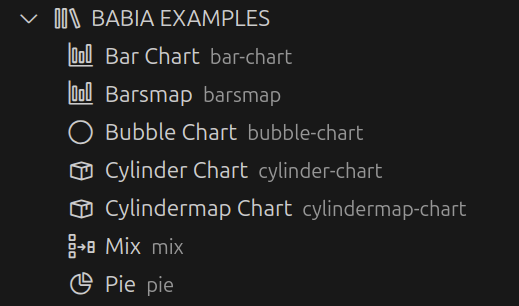
\includegraphics[width=0.55\linewidth]{img/ui-babia-examples.png}
\caption{Vista del apartado \emph{Babia Examples} mostrando la galería de ejemplos BabiaXR disponibles, cada uno lanzable con un clic y con integración completa en el ecosistema de servidores de Code-XR.}
\label{fig:ui-babia-examples}
\end{figure}

En síntesis, \emph{Babia Examples} representa una implementación madura de galería interactiva que combina descubrimiento automático, validación robusta, integración ecosistémica transparente y experiencia de usuario optimizada, proporcionando a los desarrolladores una plataforma efectiva para explorar, aprender y experimentar con las capacidades de visualización XR de BabiaXR dentro del flujo de trabajo familiar de VS Code.

%---------------------------
% Visualize Data
%---------------------------

\subsection{Visualize Data — del JSON a una visualización XR}
\label{sec:visualize-data}

El subsistema \emph{Visualize Data} constituye el núcleo de transformación de datos de Code-XR, proporcionando un pipeline sofisticado que convierte ficheros \texttt{JSON} arbitrarios en visualizaciones inmersivas BabiaXR a través de un flujo de trabajo guiado e intuitivo. Este módulo actúa como el puente principal entre datos en bruto y experiencias WebXR/AR/VR, implementando análisis automático de campos, mapeo inteligente de dimensiones, validación exhaustiva y generación de plantillas HTML completas.

El sistema se estructura en un flujo progresivo de cuatro etapas que guían al usuario desde la selección inicial del tipo de gráfico hasta el lanzamiento de un servidor local con la visualización completamente funcional, integrándose de manera transparente con la infraestructura de servidores establecida y heredando automáticamente las preferencias estéticas definidas en \emph{Visualization Settings}.

\paragraph{Arquitectura y diseño modular}
La implementación sigue una arquitectura de responsabilidades distribuidas bajo \texttt{src/visualize\_data/}, organizando el código en capas especializadas: gestión de estado (\texttt{state/}), modelos de datos (\texttt{model/}), lógica de ejecución (\texttt{runtime/}), comandos VS Code (\texttt{commands/}) y componentes de interfaz (\texttt{views/}). Esta separación permite un mantenimiento escalable y facilita la extensión futura del sistema con nuevos tipos de gráficos y fuentes de datos.

El estado del flujo de trabajo se persiste a nivel de workspace, garantizando que las configuraciones intermedias se mantengan entre sesiones de trabajo mientras el usuario experimenta con diferentes combinaciones de datos y parámetros de visualización.

\paragraph{Catálogo de tipos de gráfico}
El selector de gráficos presenta un catálogo dinámico de tipos de visualización BabiaXR, cada uno especializado en diferentes modalidades de representación de datos: gráficos de barras (\emph{Bar}), diagramas de sectores (\emph{Pie}, \emph{Donut}), visualizaciones de burbujas (\emph{Bubbles}), representaciones cilíndricas 3D (\emph{Cylinders}), mapas de barras sobre superficies (\emph{Barsmap}), distribuciones cilíndricas espaciales (\emph{Cylindermap}) y composiciones híbridas (\emph{Boats}). Cada tipo de gráfico define un conjunto específico de dimensiones requeridas y opcionales (p.\,ej., \texttt{key}, \texttt{size}, \texttt{color}, \texttt{height}) junto con su plantilla HTML/A-Frame asociada.

% TODO: Capturar screenshot del selector de gráficos mostrando la lista completa
% con iconos y descripciones de cada tipo disponible
% Nombre sugerido: ui-chart-type-selector-complete.png
\begin{figure}[H]
\centering
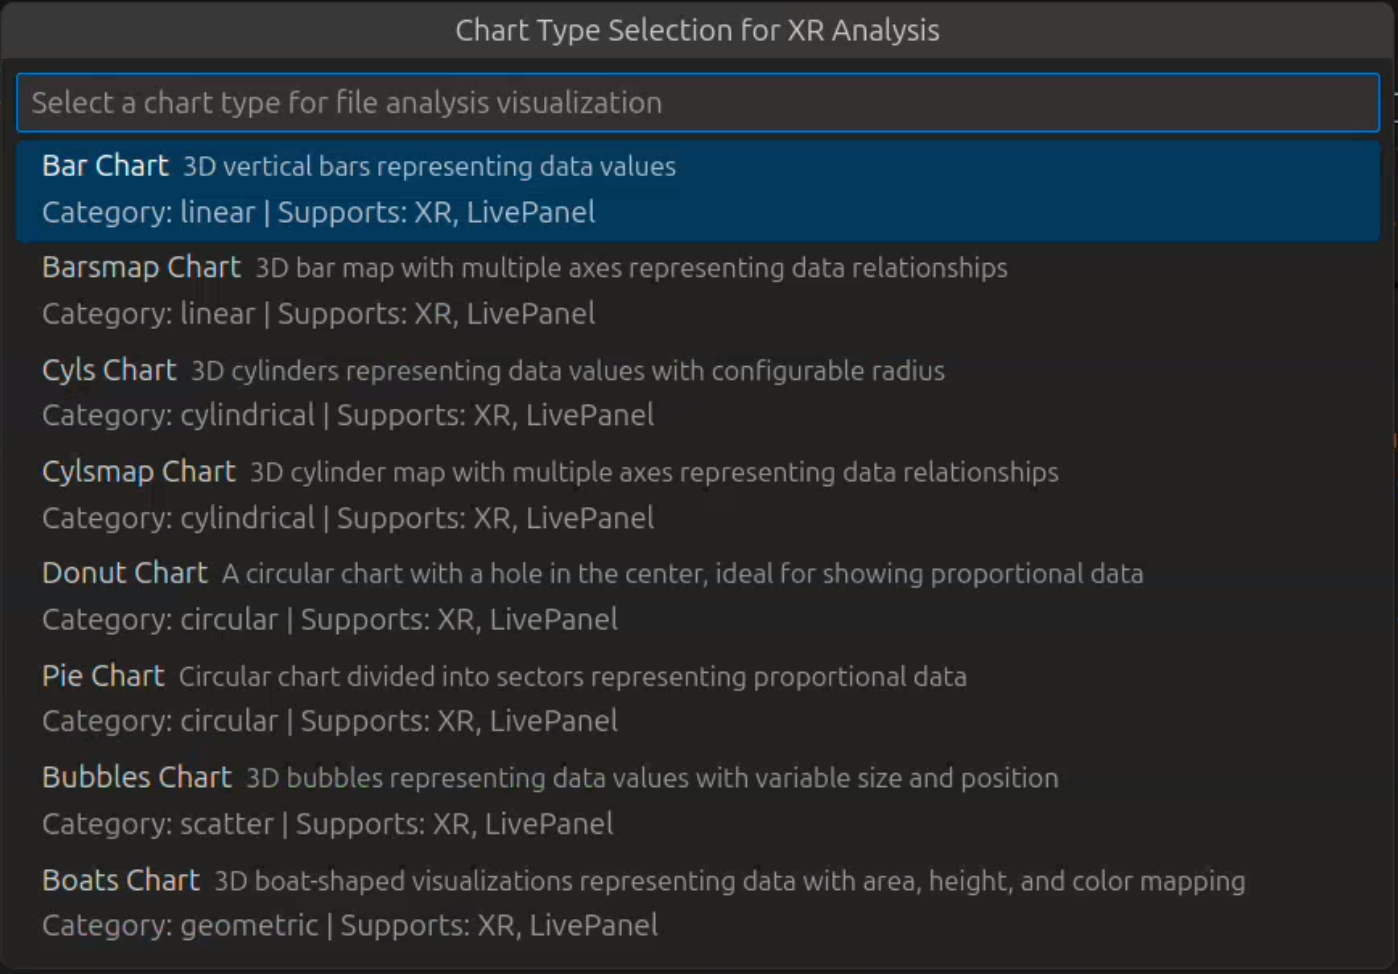
\includegraphics[width=0.58\linewidth]{img/graficos_babiaxr.png}
\caption{Selector de gráficos disponibles en \emph{Visualize Data}, mostrando la diversidad de tipos de visualización BabiaXR soportados.}
\label{fig:visualize-chart-selector}
\end{figure}

\paragraph{Análisis inteligente de datos JSON}
Una vez seleccionado el tipo de gráfico, el sistema implementa un analizador de datos JSON sofisticado que examina exhaustivamente la estructura y contenido del fichero seleccionado. El proceso de análisis detecta automáticamente los tipos de campo (\emph{string}, \emph{number}, \emph{boolean}, \emph{object}, \emph{array}), identifica campos numéricos mediante validación estricta, recopila valores de muestra para cada campo y calcula estadísticas de completitud de datos.

Esta información se presenta al usuario en forma de resumen estructurado que incluye el número total de registros, la lista de campos disponibles con sus tipos detectados y ejemplos de valores, permitiendo una toma de decisiones informada durante el proceso de mapeo de dimensiones.

\paragraph{Mapeo de dimensiones con validación contextual}
El proceso de mapeo de dimensiones constituye el corazón del sistema de transformación, permitiendo al usuario asignar campos específicos del JSON a las dimensiones requeridas por el tipo de gráfico seleccionado. El sistema implementa validación contextual inteligente: las dimensiones que requieren datos numéricos (como \texttt{size} o \texttt{height}) filtran automáticamente la lista de campos disponibles para mostrar únicamente aquellos identificados como numéricos durante el análisis previo.

La interfaz proporciona retroalimentación en tiempo real sobre el estado de configuración, destacando dimensiones obligatorias sin mapear, alertando sobre reutilización de campos en múltiples dimensiones y validando la coherencia general del mapeo antes de permitir el lanzamiento de la visualización.

% TODO: Capturar screenshot del proceso de mapeo de dimensiones mostrando:
% - Lista de dimensiones del gráfico (key, size, color, etc.)
% - Dropdown de campos JSON filtrados por tipo
% - Indicadores de validación (required, optional, warnings)
% Nombre sugerido: ui-dimension-mapping-process.png
\begin{figure}[H]
\centering
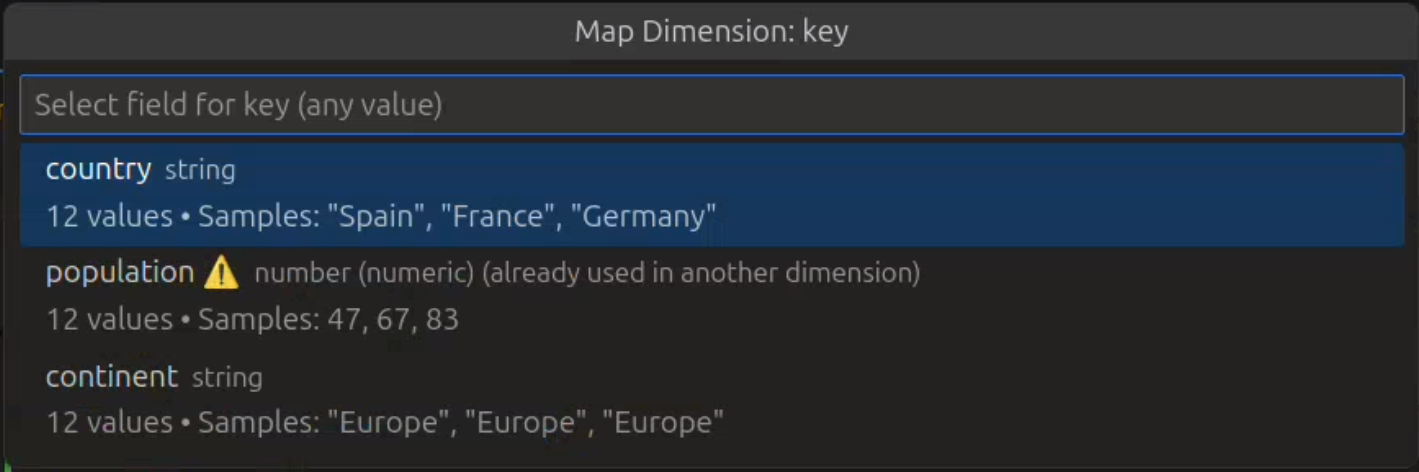
\includegraphics[width=0.80\linewidth]{img/ui-dimension-mapping-process.png}
\caption{Interfaz de mapeo de dimensiones con validación contextual, mostrando la asignación de campos JSON a dimensiones del gráfico con filtrado por tipo de dato.}
\label{fig:ui-dimension-mapping-process}
\end{figure}

\paragraph{Generación de plantillas y persistencia inteligente}
Una vez completado el mapeo, el sistema orquesta un proceso de generación sofisticado que combina la plantilla HTML del tipo de gráfico seleccionado con los datos mapeados y las preferencias de \emph{Visualization Settings}. El motor de plantillas inyecta automáticamente la configuración de paleta de colores, ambiente visual, configuración de suelo e iluminación en la escena A-Frame resultante.

Cada visualización generada se almacena de forma persistente en el \texttt{globalStorage} de VS Code bajo una estructura de directorios única que combina el nombre proporcionado por el usuario con un nonce criptográfico de 8 bytes (\texttt{Poblacion\_Continentes\_40d691b270d179f1}), garantizando unicidad y previniendo conflictos de nombres. Cada directorio contiene \texttt{index.html} (la visualización completa lista para servir) y \texttt{data.json} (copia local de los datos originales).

\paragraph{Browse Visualizations: gestión de biblioteca personal}
El apartado \emph{Browse Visualizations} proporciona una interfaz de gestión completa para la biblioteca personal de visualizaciones del usuario. El sistema escanea automáticamente el \texttt{globalStorage} para descubrir visualizaciones previamente creadas, valida la integridad de los archivos requeridos y presenta una lista organizada con opciones de relanzamiento individual y limpieza masiva mediante \emph{Reset All}.

Esta funcionalidad transforma \emph{Visualize Data} en una herramienta de uso recurrente donde los usuarios pueden mantener una colección personal de visualizaciones reutilizables, experimentar con diferentes configuraciones y compartir visualizaciones mediante el sistema de servidores integrado.

% TODO: Capturar screenshot de la sección Browse Visualizations mostrando:
% - Lista de visualizaciones almacenadas con nombres únicos
% - Botones de acción (Launch, Reset All)
% - Indicadores de estado de archivos (válidos/inválidos)
% Nombre sugerido: ui-browse-visualizations-library.png
\begin{figure}[H]
\centering
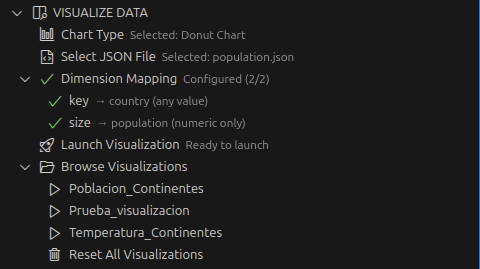
\includegraphics[width=0.70\linewidth]{img/ui-visualize-data.png}
\caption{Interfaz completa de \emph{Visualize Data} mostrando el flujo de trabajo paso a paso y la gestión de biblioteca de visualizaciones almacenadas.}
\label{fig:ui-visualize-data}
\end{figure}

\paragraph{Integración ecosistémica y herencia de configuración}
El subsistema se integra de manera transparente con el ecosistema completo de Code-XR, delegando el lanzamiento de servidores al \texttt{MultiServerLauncher} para garantizar consistencia en el comportamiento de red (HTTP/HTTPS, selección automática de puertos, apertura en panel o navegador) y registrando automáticamente cada visualización en el registro de \emph{Active Servers} con nombres personalizados que facilitan la identificación.

La herencia automática de configuración desde \emph{Visualization Settings} garantiza que todas las visualizaciones generadas respeten las preferencias estéticas del usuario sin requerir configuración adicional, aplicando de forma consistente paletas de colores, ambientes XR, configuración de suelo e iluminación a través de la integración con el motor de plantillas centralizado.

\paragraph{Validación robusta y prevención de errores}
El sistema implementa un esquema de validación multicapa que abarca desde la validación de formato JSON hasta la prevención de lanzamientos duplicados. El analizador de JSON maneja graciosamente archivos malformados, datasets de gran tamaño y estructuras de datos complejas, mientras que el validador de mapeo de dimensiones previene configuraciones incompletas o inconsistentes.

La prevención de duplicados opera tanto a nivel de campos (alertando sobre reutilización en múltiples dimensiones) como a nivel de servidores activos (evitando el lanzamiento de visualizaciones ya en ejecución), proporcionando una experiencia de usuario fluida y libre de conflictos. Los mensajes de error contextuales guían al usuario hacia la resolución de problemas específicos, mientras que la habilitación/deshabilitación dinámica de controles UI mantiene la coherencia del flujo de trabajo.


%---------------------------
% Visualization Settings
%---------------------------

\subsection{Visualization Settings}
\label{sec:visualization-settings}

El apartado \emph{Visualization Settings} constituye el sistema de configuración visual global de Code-XR, permitiendo personalizar cuatro aspectos fundamentales que se aplicarán automáticamente a todas las visualizaciones generadas: \textbf{color de fondo}, \textbf{color del suelo}, \textbf{preset del entorno} y \textbf{paleta de gráficos}. Este módulo se integra como una sección adicional en el árbol principal de la extensión, proporcionando una interfaz intuitiva para la gestión de preferencias visuales persistentes.

\paragraph{Arquitectura y persistencia de configuración}
El subsistema sigue una arquitectura modular distribuida en capas especializadas bajo \texttt{src/visualization\_settings/}, implementando separación clara entre modelo de datos (\texttt{model/}), almacenamiento (\texttt{storage/}), comandos (\texttt{commands/}), vistas (\texttt{views/}) y utilidades (\texttt{utils/}). La persistencia se gestiona mediante un sistema de doble capa: almacenamiento primario en fichero JSON ubicado en el \texttt{globalStorage} de VS Code (\texttt{visualization-settings.json}) y respaldo en \texttt{globalState} para compatibilidad con versiones anteriores.

Esta aproximación garantiza que las configuraciones se mantengan entre sesiones y workspaces, con migración automática desde el sistema legacy y validación estricta de formatos. El fichero de configuración emplea una estructura simplificada que mapea los cuatro parámetros visuales:

\begin{figure}[H]
\centering
\begin{minipage}{0.9\linewidth}
\begin{lstlisting}[language=json,
caption={Estructura del archivo \texttt{visualization-settings.json} que persiste las preferencias visuales globales.},
label={fig:visualization-settings-json}]
{
  "backgroundColor": "#FFFFFF",
  "groundColor": "#000000",
  "environment": "forest", 
  "palette": "ubuntu"
}
\end{lstlisting}
\end{minipage}
\end{figure}

\paragraph{Interfaz de usuario y experiencia visual}
La sección \emph{Visualization Settings} se presenta como un apartado colapsible dentro del árbol principal de Code-XR, exponiendo cada parámetro como un elemento interactivo con iconografía contextual diferenciada. Los parámetros \emph{Background Color} y \emph{Ground Color} muestran muestras de color generadas dinámicamente como iconos SVG de 16×16 píxeles que reflejan visualmente el color seleccionado, mientras que \emph{Environment Preset} utiliza un icono de globo terráqueo y \emph{Chart Palette} emplea un símbolo de paleta artística. Esta representación visual permite al usuario identificar rápidamente el estado actual de su configuración sin necesidad de navegar por los paneles de ajuste.

% TODO: Capturar screenshot del apartado Visualization Settings en el árbol de Code-XR 
% mostrando los 4 elementos con sus iconos dinámicos de color
% Nombre sugerido: ui-visualization-settings-tree.png
\begin{figure}[H]
\centering
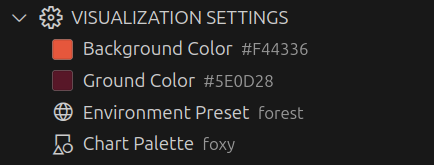
\includegraphics[width=0.60\linewidth]{img/ui-visualization-settings-tree.png}
\caption{Vista del apartado \emph{Visualization Settings} integrado en el árbol principal, mostrando iconos dinámicos de color para los parámetros visuales.}
\label{fig:ui-visualization-settings-tree}
\end{figure}

\paragraph{Flujo de configuración de colores}
La configuración de colores (\emph{Background} y \emph{Ground}) implementa un flujo híbrido que prioriza la experiencia nativa del navegador. Al hacer clic en cualquiera de estos parámetros, el sistema despliega un panel webview personalizado que integra el selector de color HTML5 nativo, proporcionando una interfaz familiar con preview en tiempo real y validación automática del formato hexadecimal (\texttt{\#RRGGBB}).

% TODO: Capturar screenshot del panel de selección de colores (webview) 
% mostrando el color picker HTML5 con el color actual seleccionado
% Nombre sugerido: ui-color-picker-panel.png
\begin{figure}[H]
\centering
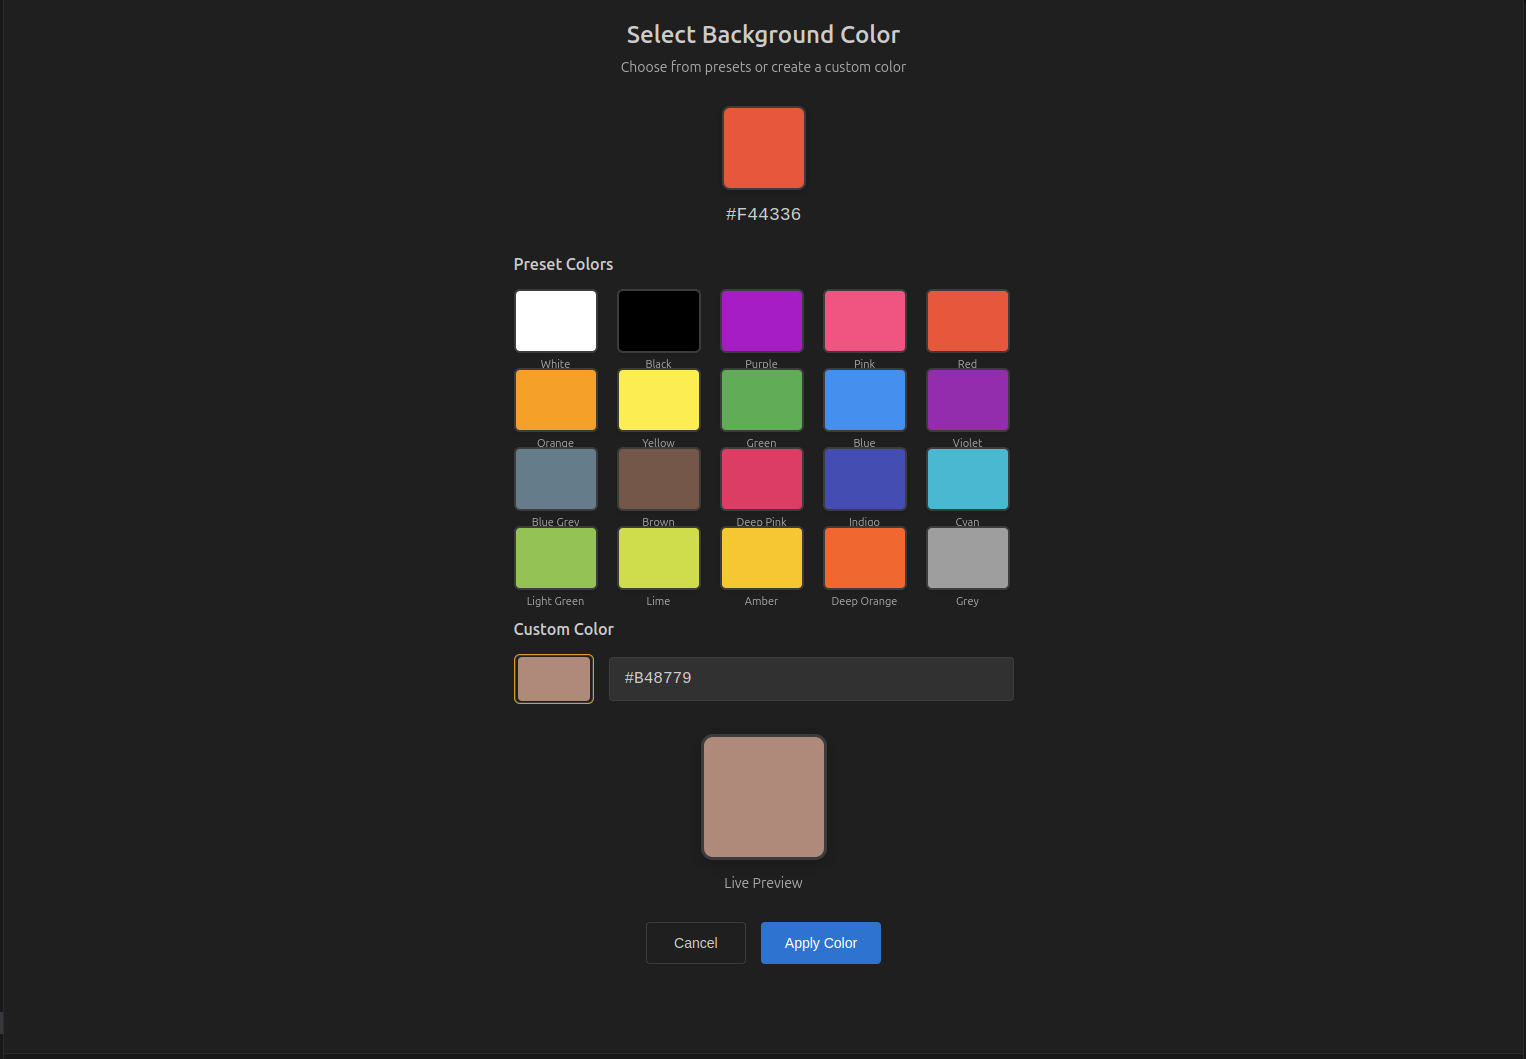
\includegraphics[width=1\linewidth]{img/ui-color-picker-panel.png}
\caption{Panel de selección de colores mediante webview integrado, utilizando el selector HTML5 nativo con validación en tiempo real.}
\label{fig:ui-color-picker-panel}
\end{figure}

Como alternativa de respaldo, el sistema ofrece un flujo basado en \emph{QuickPick} que presenta una selección de colores predefinidos junto con la opción de introducir valores hexadecimales personalizados. Este mecanismo incluye validación con reintentos (hasta 3 intentos) y mensajes contextuales que guían al usuario hacia el formato correcto.

\paragraph{Configuración de entornos y paletas}
Los parámetros \emph{Environment Preset} y \emph{Chart Palette} emplean una interfaz de selección mediante \emph{QuickPick} que presenta las opciones disponibles con etiquetas descriptivas y contextuales. El catálogo de entornos abarca 12 presets predefinidos de A-Frame (\texttt{forest}, \texttt{tron}, \texttt{egypt}, \texttt{dream}, \texttt{volcano}, \texttt{arches}, etc.) que redefinen completamente la ambientación visual y atmosférica de las escenas XR, desde bosques realistas hasta paisajes futuristas estilo \emph{Tron}. Paralelamente, las paletas de gráficos proporcionan 9 esquemas cromáticos especializados de BabiaXR (\texttt{ubuntu}, \texttt{blues}, \texttt{sunset}, \texttt{foxy}, \texttt{icecream}, etc.), cada uno optimizado para diferentes contextos de visualización y tipos de datos.

% TODO: Capturar screenshot del QuickPick de Environment Preset
% mostrando la lista de entornos disponibles (forest, tron, egypt, etc.) 
% Nombre sugerido: ui-environment-preset-quickpick.png
\begin{figure}[H]
\centering
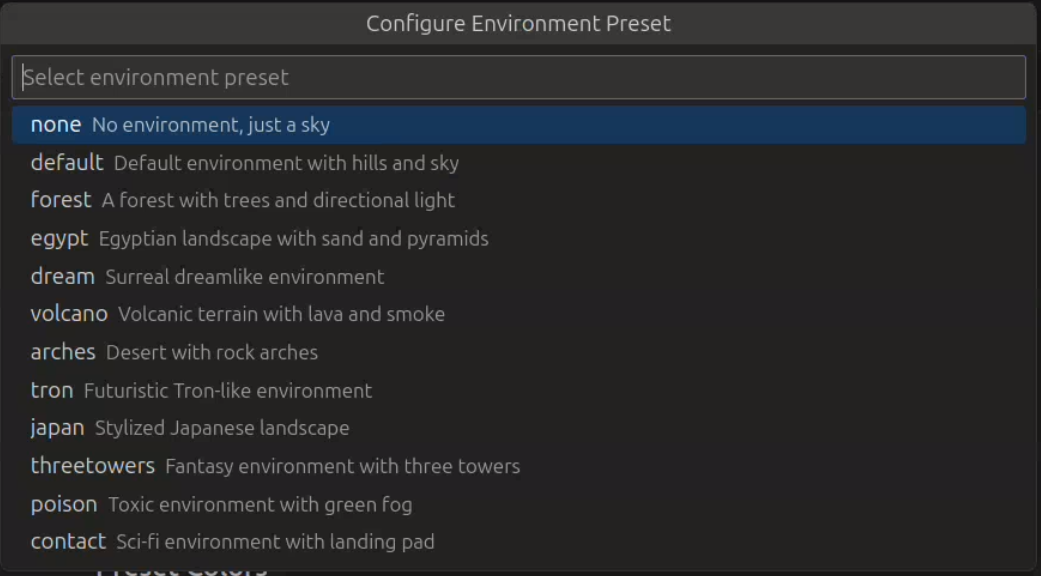
\includegraphics[width=0.70\linewidth]{img/ui-environment-preset-quickpick.png}
\caption{Selector \emph{QuickPick} para \emph{Environment Preset}, mostrando la gama de entornos A-Frame disponibles con descripciones contextuales.}
\label{fig:ui-environment-preset-quickpick}
\end{figure}

% TODO: Capturar screenshot del QuickPick de Chart Palette
% mostrando la lista de paletas disponibles (ubuntu, blues, sunset, etc.)
% Nombre sugerido: ui-chart-palette-quickpick.png
\begin{figure}[H]
\centering
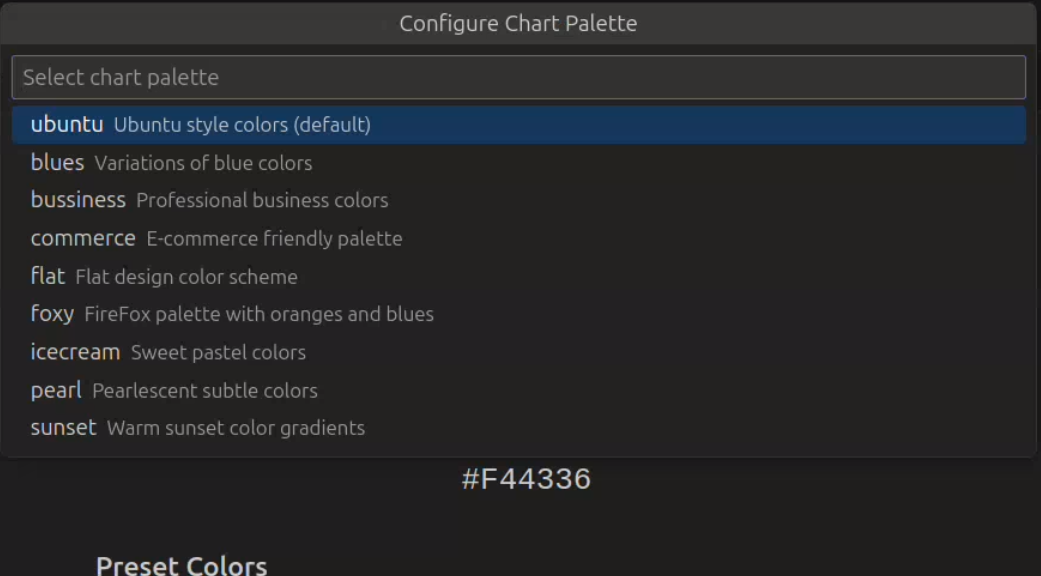
\includegraphics[width=0.70\linewidth]{img/ui-chart-palette-quickpick.png}
\caption{Selector \emph{QuickPick} para \emph{Chart Palette}, mostrando las paletas de colores BabiaXR con vistas previas.}
\label{fig:ui-chart-palette-quickpick}
\end{figure}

\paragraph{Aplicación automática en visualizaciones}
La verdadera potencia de \emph{Visualization Settings} reside en su integración transparente con el motor de plantillas de Code-XR. Cada vez que se genera una visualización (ya sea desde \emph{Babia Examples}, \emph{Visualize Data} o análisis de código), el sistema invoca automáticamente \texttt{getVisualizationConfiguration()}, que recupera las preferencias activas y las inyecta en las plantillas HTML/A-Frame correspondientes.

Este proceso de sustitución mapea cada parámetro a atributos específicos de los componentes:
\begin{itemize}
\item \textbf{Background Color} $\rightarrow$ atributo \texttt{background="color: \#FFFFFF"} de la escena A-Frame
\item \textbf{Environment Preset} $\rightarrow$ componente \texttt{environment="preset: forest"} 
\item \textbf{Ground Color} $\rightarrow$ parámetro \texttt{groundColor: \#000000} del entorno
\item \textbf{Chart Palette} $\rightarrow$ atributo \texttt{palette: ubuntu} en componentes BabiaXR
\end{itemize}

\paragraph{Iconografía dinámica y representación visual}
Una característica particularmente distintiva del sistema es la generación automática de iconos SVG que funcionan como indicadores visuales directos en la interfaz de usuario. Para los parámetros \emph{Background Color} y \emph{Ground Color}, la extensión genera dinámicamente pequeños cuadrados de color de 16×16 píxeles que se muestran como iconos junto a cada elemento en el árbol de Code-XR, permitiendo al usuario identificar de un vistazo qué colores tiene configurados sin necesidad de abrir los paneles de configuración.

Estos iconos SVG se crean bajo demanda cada vez que el usuario modifica un color, aplicando efectos sutiles de borde y sombra interior para garantizar la legibilidad sobre diferentes temas de VS Code (claro y oscuro). La nomenclatura empleada (\texttt{\{settingKey\}\_\{hexcolor\}.svg}) permite un sistema de caché eficiente: si el usuario vuelve a seleccionar un color previamente usado, el icono se reutiliza en lugar de regenerarse. El sistema implementa limpieza automática de iconos obsoletos cuando se cambian los valores, evitando la acumulación progresiva de archivos temporales en el \texttt{globalStorage}.

\paragraph{Validación y robustez del sistema}
El subsistema implementa un esquema de validación multicapa que garantiza la integridad de la configuración: validación estricta de formato hexadecimal para colores mediante expresión regular (\texttt{/\^\#[0-9a-fA-F]\{6\}\$/}), verificación de correspondencia de presets con los catálogos oficiales de A-Frame y BabiaXR, y mecanismos de recuperación automática que restauran valores por defecto ante configuraciones corrompidas o incompatibles. La experiencia de usuario se complementa con retroalimentación contextual mediante mensajes informativos, indicadores visuales de estado y deshabilitación inteligente de controles según el flujo de configuración activo.

Esta aproximación de validación progresiva, combinada con la persistencia dual y la integración transparente con el motor de plantillas, posiciona a \emph{Visualization Settings} como un sistema maduro y confiable que equilibra flexibilidad de personalización con robustez operacional, proporcionando a los usuarios un control granular y consistente sobre la estética de todas las visualizaciones XR generadas por Code-XR.


%
%%%%%%%%%%%%%%%%%%%%%%%%%%%%%%%%%%%%%%%%%%%%%%%%%%%%%%%%%%%%%%%%%%%%%%%%%%%%%%%%
%%%%%%%%%%%%%%%%%%%%%%%%%%%%%%%%%%%%%%%%%%%%%%%%%%%%%%%%%%%%%%%%%%%%%%%%%%%%%%%%
% EXPERIMENTOS Y VALIDACIÓN %
%%%%%%%%%%%%%%%%%%%%%%%%%%%%%%%%%%%%%%%%%%%%%%%%%%%%%%%%%%%%%%%%%%%%%%%%%%%%%%%%

\cleardoublepage
\chapter{Experimentos y validación}
\label{chap:experimentos}

Este capítulo se introdujo como requisito en 2019. 
Describe los experimentos y casos de test que tuviste que implementar para validar tus resultados. 
Incluye también los resultados de validación que permiten afirmar que tus resultados son correctos. 


%%%%%%%%%%%%%%%%%%%%%%%%%%%%%%%%%%%%%%%%%%%%%%%%%%%%%%%%%%%%%%%%%%%%%%%%%%%%%%%%
%%%%%%%%%%%%%%%%%%%%%%%%%%%%%%%%%%%%%%%%%%%%%%%%%%%%%%%%%%%%%%%%%%%%%%%%%%%%%%%%
% RESULTADOS %
%%%%%%%%%%%%%%%%%%%%%%%%%%%%%%%%%%%%%%%%%%%%%%%%%%%%%%%%%%%%%%%%%%%%%%%%%%%%%%%%

\cleardoublepage
\chapter{Resultados}
\label{chap:resultados}

En este capítulo se incluyen los resultados de tu trabajo fin de grado.

Si es una herramienta de análisis lo que has realizado, aquí puedes poner ejemplos de haberla utilizado para que se vea su utilidad.


%%%%%%%%%%%%%%%%%%%%%%%%%%%%%%%%%%%%%%%%%%%%%%%%%%%%%%%%%%%%%%%%%%%%%%%%%%%%%%%%
%%%%%%%%%%%%%%%%%%%%%%%%%%%%%%%%%%%%%%%%%%%%%%%%%%%%%%%%%%%%%%%%%%%%%%%%%%%%%%%%
% CONCLUSIONES %
%%%%%%%%%%%%%%%%%%%%%%%%%%%%%%%%%%%%%%%%%%%%%%%%%%%%%%%%%%%%%%%%%%%%%%%%%%%%%%%%

\cleardoublepage
\chapter{Conclusiones}
\label{chap:conclusiones}


\section{Consecución de objetivos}
\label{sec:consecucion-objetivos}

Esta sección es la sección espejo de las dos primeras del capítulo de objetivos, donde se planteaba el objetivo general y se elaboraban los específicos.

Es aquí donde hay que debatir qué se ha conseguido y qué no. 
Cuando algo no se ha conseguido, se ha de justificar, en términos de qué problemas se han encontrado y qué medidas se han tomado para mitigar esos problemas.

Y si has llegado hasta aquí, siempre es bueno pasarle el corrector ortográfico, que las erratas quedan fatal en la memoria final.
Para eso, en Linux tenemos aspell, que se ejecuta de la siguiente manera desde la línea de \emph{shell}:

\begin{verbatim}
  aspell --lang=es_ES -c memoria.tex
\end{verbatim}

\section{Aplicación de lo aprendido}
\label{sec:aplicacion}

Aquí viene lo que has aprendido durante el Grado/Máster y que has aplicado en el TFG/TFM.
Una buena idea es poner las asignaturas más relacionadas y comentar en un párrafo los conocimientos y habilidades puestos en práctica.

\begin{enumerate}
  \item a
  \item b
\end{enumerate}


\section{Lecciones aprendidas}
\label{sec:lecciones_aprendidas}

Aquí viene lo que has aprendido en el Trabajo Fin de Grado/Máster.

\begin{enumerate}
  \item Aquí viene uno.
  \item Aquí viene otro.
\end{enumerate}


\section{Trabajos futuros}
\label{sec:trabajos_futuros}

Ningún proyecto ni software se termina, así que aquí vienen ideas y funcionalidades que estaría bien tener implementadas en el futuro.

Es un apartado que sirve para dar ideas de cara a futuros TFGs/TFMs.


%%%%%%%%%%%%%%%%%%%%%%%%%%%%%%%%%%%%%%%%%%%%%%%%%%%%%%%%%%%%%%%%%%%%%%%%%%%%%%%%
%%%%%%%%%%%%%%%%%%%%%%%%%%%%%%%%%%%%%%%%%%%%%%%%%%%%%%%%%%%%%%%%%%%%%%%%%%%%%%%%
% APÉNDICE(S) %
%%%%%%%%%%%%%%%%%%%%%%%%%%%%%%%%%%%%%%%%%%%%%%%%%%%%%%%%%%%%%%%%%%%%%%%%%%%%%%%%

\cleardoublepage
\appendix
\chapter{Manual de usuario}
\label{app:manual}

Esto es un apéndice.
Si has creado una aplicación, siempre viene bien tener un manual de usuario.
Pues ponlo aquí.

%%%%%%%%%%%%%%%%%%%%%%%%%%%%%%%%%%%%%%%%%%%%%%%%%%%%%%%%%%%%%%%%%%%%%%%%%%%%%%%%
%%%%%%%%%%%%%%%%%%%%%%%%%%%%%%%%%%%%%%%%%%%%%%%%%%%%%%%%%%%%%%%%%%%%%%%%%%%%%%%%
% BIBLIOGRAFIA %
%%%%%%%%%%%%%%%%%%%%%%%%%%%%%%%%%%%%%%%%%%%%%%%%%%%%%%%%%%%%%%%%%%%%%%%%%%%%%%%%

\cleardoublepage

% Las siguientes dos instrucciones es todo lo que necesitas
% para incluir las citas en la memoria
\bibliographystyle{abbrv}
\bibliography{memoria}  % memoria.bib es el nombre del fichero que contiene
% las referencias bibliográficas. Abre ese fichero y mira el formato que tiene,
% que se conoce como BibTeX. Hay muchos sitios que exportan referencias en
% formato BibTeX. Prueba a buscar en http://scholar.google.com por referencias
% y verás que lo puedes hacer de manera sencilla.
% Más información: 
% http://texblog.org/2014/04/22/using-google-scholar-to-download-bibtex-citations/

\end{document}
